\documentclass[justified]{tufte-book}

% ams
\usepackage{amssymb,amsmath}

\usepackage{ifxetex,ifluatex}
\usepackage{fixltx2e} % provides \textsubscript
\ifnum 0\ifxetex 1\fi\ifluatex 1\fi=0 % if pdftex
  \usepackage[T1]{fontenc}
  \usepackage[utf8]{inputenc}
\else % if luatex or xelatex
  \makeatletter
  \@ifpackageloaded{fontspec}{}{\usepackage{fontspec}}
  \makeatother
  \defaultfontfeatures{Ligatures=TeX,Scale=MatchLowercase}
  \makeatletter
  \@ifpackageloaded{soul}{
     \renewcommand\allcapsspacing[1]{{\addfontfeature{LetterSpace=15}#1}}
     \renewcommand\smallcapsspacing[1]{{\addfontfeature{LetterSpace=10}#1}}
   }{}
  \makeatother

\fi

% graphix
\usepackage{graphicx}
\setkeys{Gin}{width=\linewidth,totalheight=\textheight,keepaspectratio}

% booktabs
\usepackage{booktabs}

% url
\usepackage{url}

% hyperref
\usepackage{hyperref}

% units.
\usepackage{units}


\setcounter{secnumdepth}{2}

% citations

% pandoc syntax highlighting

% longtable
\usepackage{longtable,booktabs}

% multiplecol
\usepackage{multicol}

% strikeout
\usepackage[normalem]{ulem}

% morefloats
\usepackage{morefloats}


% tightlist macro required by pandoc >= 1.14
\providecommand{\tightlist}{%
  \setlength{\itemsep}{0pt}\setlength{\parskip}{0pt}}

% title / author / date
\title{Curriculum vitae}
\author{19/08/1992}
\date{}

%\usepackage{MinionPro}
%\usepackage{fontspec}
%\newfontfamily\DejaSans{DejaVu Sans}

\newcommand{\given}{\mid}
\renewcommand{\neg}{\mathbin{\sim}}
\renewcommand{\wedge}{\mathbin{\&}}
\renewcommand{\u}{U}
\newcommand{\gt}{>}
\newcommand{\p}{Pr}
\newcommand{\E}{E}
\newcommand{\EU}{EU}
\newcommand{\pr}{Pr}
\newcommand{\po}{Pr^*}
\definecolor{bookred}{RGB}{228,6,19}
\definecolor{bookblue}{RGB}{0,92,169}
\definecolor{bookpurple}{RGB}{114,49,94}

\newenvironment{epigraph}%
{
\begin{flushright}    
\begin{minipage}{20em}
\begin{flushright}
\itshape
}%
{
\end{flushright}
\end{minipage}
\end{flushright}
}
\newenvironment{problem}{\begin{quote}\normalsize}{\end{quote}}
\newenvironment{puzzle}{\begin{quote}\normalsize}{\end{quote}}
\newenvironment{argument}{\begin{quote}\normalsize}{\end{quote}}
\usepackage{fontawesome}
\newenvironment{warning}{\begin{itemize}\item[\faBan]}{\end{itemize}}
\usepackage{marvosym}
\newenvironment{info}{\begin{itemize}\item[\Info]}{\end{itemize}}

%%%% Kevin Godny's code for title page and contents from https://groups.google.com/forum/#!topic/tufte-latex/ujdzrktC1BQ
\makeatletter
\renewcommand{\maketitlepage}{%
\begingroup%
\setlength{\parindent}{0pt}
{\fontsize{18}{18}\selectfont\textit{\ © Jan. 2020}\par}
\vspace{1.75in}{\fontsize{36}{14}\selectfont\@title\par}
\vspace{0.5in}{\fontsize{20}{14}\selectfont Falnésio Ghander Soares Borges\par}
\vspace{0.5in}{\fontsize{14}{14}\selectfont\textsf{\smallcaps{Falnesio.ghander@economia.ufjf.br}}\par}
\vspace{0.5in}{\fontsize{14}{14}\selectfont\textsf{\smallcaps{(33) 9 2000-5046}}\par}
\vfill{\fontsize{14}{14}\selectfont\textit{19/08/1992}\par}
\thispagestyle{empty}
\endgroup
}
\makeatother

% Change shape from [display] to [block] to keep chapter numbers and titles on the same line
\titleformat{\chapter}%
  [block]% shape
  {\relax\ifthenelse{\NOT\boolean{@tufte@symmetric}}{\begin{fullwidth}}{}}% format applied to label+text
  {\itshape\huge\thechapter}% label
  {3em}% horizontal separation between label and title body
  {\huge\rmfamily\itshape}% before the title body
  [\ifthenelse{\NOT\boolean{@tufte@symmetric}}{\end{fullwidth}}{}]% after the title body


\usepackage{etoolbox}
% Jesse Rosenthal's code from https://groups.google.com/forum/#!topic/pandoc-discuss/wCF78X6SvwY
% Avoid new pagraph/indent after lists, quotes, etc.
\makeatletter
\newcommand{\gobblepars}{% 
    \@ifnextchar\par% 
        {\expandafter\gobblepars\@gobble}% 
        {}}
\newcommand{\eatpar}{\@ifnextchar\par{\@gobble}{}}
\newcommand{\forcepar}{\par}
\makeatother
\AfterEndEnvironment{quote}{\expandafter\gobblepars}
\AfterEndEnvironment{enumerate}{\expandafter\gobblepars}
\AfterEndEnvironment{itemize}{\expandafter\gobblepars}
\AfterEndEnvironment{description}{\expandafter\gobblepars}
\AfterEndEnvironment{example}{\expandafter\gobblepars}
\AfterEndEnvironment{argument}{\expandafter\gobblepars}
\AfterEndEnvironment{problem}{\expandafter\gobblepars}
\AfterEndEnvironment{info}{\expandafter\gobblepars}
\AfterEndEnvironment{warning}{\expandafter\gobblepars}
\AfterEndEnvironment{longtable}{\expandafter\gobblepars} % not working, why?


% prevent extra space when \newthought follows \section
% see: https://tex.stackexchange.com/questions/291746/tufte-latex-newthought-after-section
\makeatletter
\def\tuftebreak{%
  \if@nobreak\else
    \par
    \ifdim\lastskip<\tufteskipamount
      \removelastskip \penalty -100
      \tufteskip
    \fi
  \fi
}
\makeatother

% indent lists a bit
\usepackage{enumitem}
\setlist[1]{leftmargin=24pt}

\begin{document}

\maketitle



{
\setcounter{tocdepth}{1}
\tableofcontents
}

\hypertarget{section}{%
\chapter*{.}\label{section}}
\addcontentsline{toc}{chapter}{.}

\newthought{Graduado} em Ciências Econômicas na Universidade Federal de Juiz de Fora, Campus GV e participa do Núcleo de Agroecologia de Governador Valadares NAGÔ. Tem interesse em sistemas complexos. Acredita que modelos que incorporam as sutilezas da heterogeneidade social são úteis na produção de soluções democráticas mais eficazes e eficientes para demandas socioeconômicas e que o estudo econômico tem muito espaço para multidisciplinaridade na formulação de modelos simples mais próximos da realidade.

\begin{marginfigure}
    Informações de contato:
    
    \href{mailto:falnesio.ghander@economia.ufjf.br}{\nolinkurl{falnesio.ghander@economia.ufjf.br}}
    
    \href{https://t.me/falnesio}{Telegram: (33) 9 2000-5046}
    
    \href{https://www.linkedin.com/in/faln\%C3\%A9sio-g-s-borges-43b615149/}{LinkedIn}
    
    \href{http://lattes.cnpq.br/8513885038003903}{Lattes}
    
    \href{https://github.com/Falnesio}{Github}
    \end{marginfigure}

É um pesquisador muito dedicado e focado, é acostumado a entrar em projetos e iniciativas novas, se adaptando aos processos, metodologias e técnicas, aceitando desafios e sempre aprendendo. Trabalha bem em equipe e sempre busca passar o conhecimento que adquiriu para frente.

\hypertarget{habilidades-virtuais}{%
\section{Habilidades Virtuais}\label{habilidades-virtuais}}

\begin{center}\rule{0.5\linewidth}{\linethickness}\end{center}

\textbf{Linguagens}
- Português Fluente
- Inglês Fluente
- Português Fluente
- Inglês Fluente
- Inglês Fluente
- Português Fluente
- Inglês Fluente

\textbf{Linguagens de Programação}
- R
- Python
- SQL

\textbf{Softwares}
- Microsoft Excel
- Microsoft Word

A ``cheat sheet'' summarizing key definitions and formulas appears in {[}Appendix{]}{[}Cheat Sheet{]} {[}A{]}{[}Cheat Sheet{]}. Further appendices cover the axiomatic construction of probability theory, Hume's problem of induction, and Goodman's new ridle of induction.

\newthought{I} usually get a mix of students in my course, with different ideological inclinations and varying levels of background. For some the technical material is easy, even review. For others, a healthy skepticism about scientific methods and discourses comes naturally. My goal is to get these students all more or less on the same page.

By the end of the course, students with little formal background have a bevy of tools for thinking about uncertainty. They can understand much more of the statistical and scientific discourse they encounter. And hopefully they have a greater appreciation for the value of formal methods. Students who already have strong formal tools and skills will, I hope, better understand their limitations. I want them to understand why these tools leave big questions open---not just philosophically, but also in very pressing, practical ways.

\newthought{The} book was made with the \texttt{bookdown} package created by Yihui Xie. It's a wonderful tool, built on a bunch of other technologies I love, especially the R programming language and the pandoc conversion tool created by philosopher John MacFarlane. The book's visual style emulates the famous designs of Edward Tufte, thanks to more software created by Yihui Xie, J. J. Allaire, and many others who adapted Tufte's designs to HTML and PDF (via LaTeX).

If it weren't for these tools, I never would have written this book. It wouldn't have been possible to create one that does all the things this book is meant to do. I also owe inspiration to Kieran Healy's book \href{http://socviz.co/}{\emph{Data Visualization: A Practical Introduction}}, which uses the same suite of tools. It gave me the idea to use those tools for an updated, open, and visually enhanced rendition of the classic material from Skyrms and Hacking.

Finally, I'm indebted to several teaching assistants and students who helped with earlier drafts. Thanks especially to Liang Zhou Koh and Meagan Phillips, who contributed several exercises; to Soroush Marouzi and Daniel Munro, who worked out the kinks during the first semester the book was piloted; and to the students in that course, who bore with us, and contributed several corrections of their own.

\hypertarget{part-part-i}{%
\part*{Part I}\label{part-part-i}}
\addcontentsline{toc}{part}{Part I}

\hypertarget{the-monty-hall-problem}{%
\chapter{The Monty Hall Problem}\label{the-monty-hall-problem}}

\begin{epigraph}
When tackling a math problem,\\
I encourage students to \emph{draw a picture}.\\
---Francis Su
\end{epigraph}

\newthought{Imagine} you're on a game show. There are three doors, one with a prize behind it. You're allowed to pick any door, so you choose the first one at random, door A.

\begin{marginfigure}
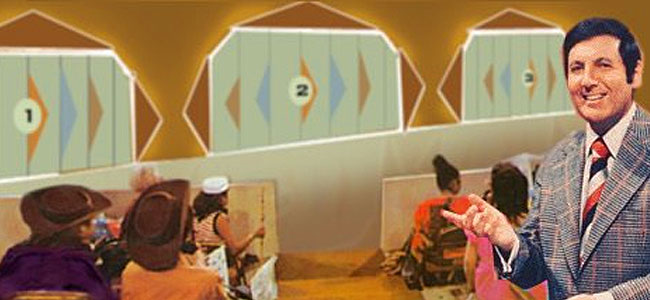
\includegraphics{img/lets_make_a_deal.png} The Monty Hall problem is
named after the creator and host of the game show \emph{Let's Make a
Deal}.
\end{marginfigure}

Now the rules of the game require the host to open one of the other doors and let you switch your choice if you want. Because the host doesn't want to give away the game, they always open an empty door.

In your case, the host opens door C: no prize, as expected. ``Do you want to switch to door B?'', the host asks.

Pause a moment to think about your answer before reading on.

\newthought{What} did you decide? Did you conclude it doesn't matter whether you stick with door A or switch to door B?

\begin{marginfigure}
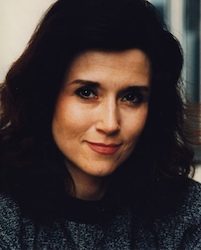
\includegraphics{img/marilyn_vos_savant.png} Marilyn vos Savant made the
Monty Hall problem famous when she solved it correctly in her ``Ask
Marilyn'' column for \emph{Parade} magazine. Read more about it in
\href{https://www.nytimes.com/1991/07/21/us/behind-monty-hall-s-doors-puzzle-debate-and-answer.html}{\emph{The
New York Times}}.
\end{marginfigure}

If so, you're in good company. Most people find this answer sensible, including some professors of statistics and mathematics. They figure there are only two possibilities remaining, door A and door B, each with the same one-in-two chance of being the winner. So it doesn't matter which one you pick.

But the right answer is you should switch. Door B is now twice as likely to be the winner as door A. Why?

The reason is subtle. One way to think about it is that the host's choice of which door to open is a bit of a tell. Maybe they \emph{had} to open door C, because the prize is behind door B and they didn't want to give that away. Of course, it could be behind door A instead, so maybe they just picked door C at random. But there was only a one-in-three chance the prize would be behind door A. Which means there's a two-in-three chance they didn't really have a choice, they had to open door C to avoid showing you the prize behind door B.

\begin{marginfigure}
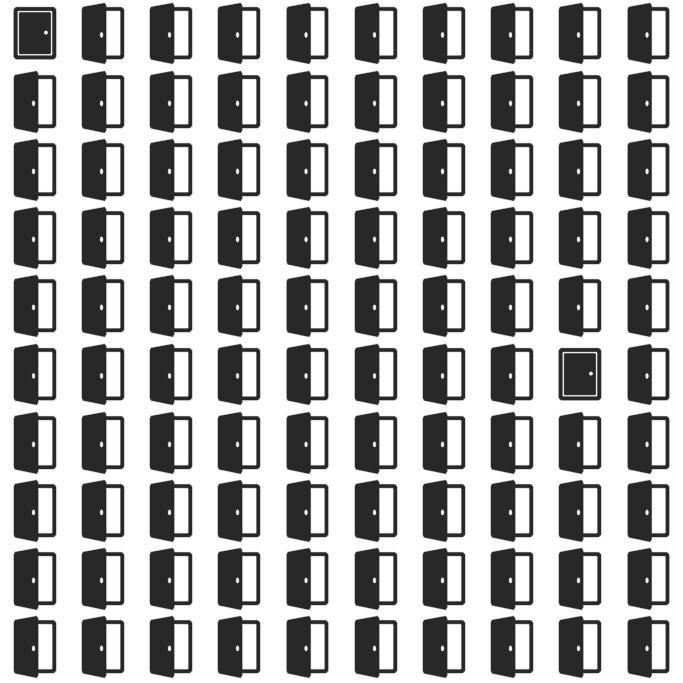
\includegraphics{_main_files/figure-latex/montygrid-1} \caption[The hundred-door version of the Monty Hall problem, suggested by Marilyn vos Savant]{The hundred-door version of the Monty Hall problem, suggested by Marilyn vos Savant}\label{fig:montygrid}
\end{marginfigure}

Here's another way to think about it. Imagine the game had a hundred doors instead of just three. And suppose again you start by picking the first door at random. Then the host opens \emph{all the other doors but one}, door \(59\) let's say. You have to ask yourself: why did they pick door \(59\) to leave closed?? Almost certainly because that's where the prize is hidden! Maybe you got really lucky and picked right with the first door at the beginning. But it's way more likely you didn't, and the host had to keep door \(59\) closed to avoid giving away the game.

\hypertarget{diagramming-the-solution}{%
\section{Diagramming the Solution}\label{diagramming-the-solution}}

\begin{marginfigure}
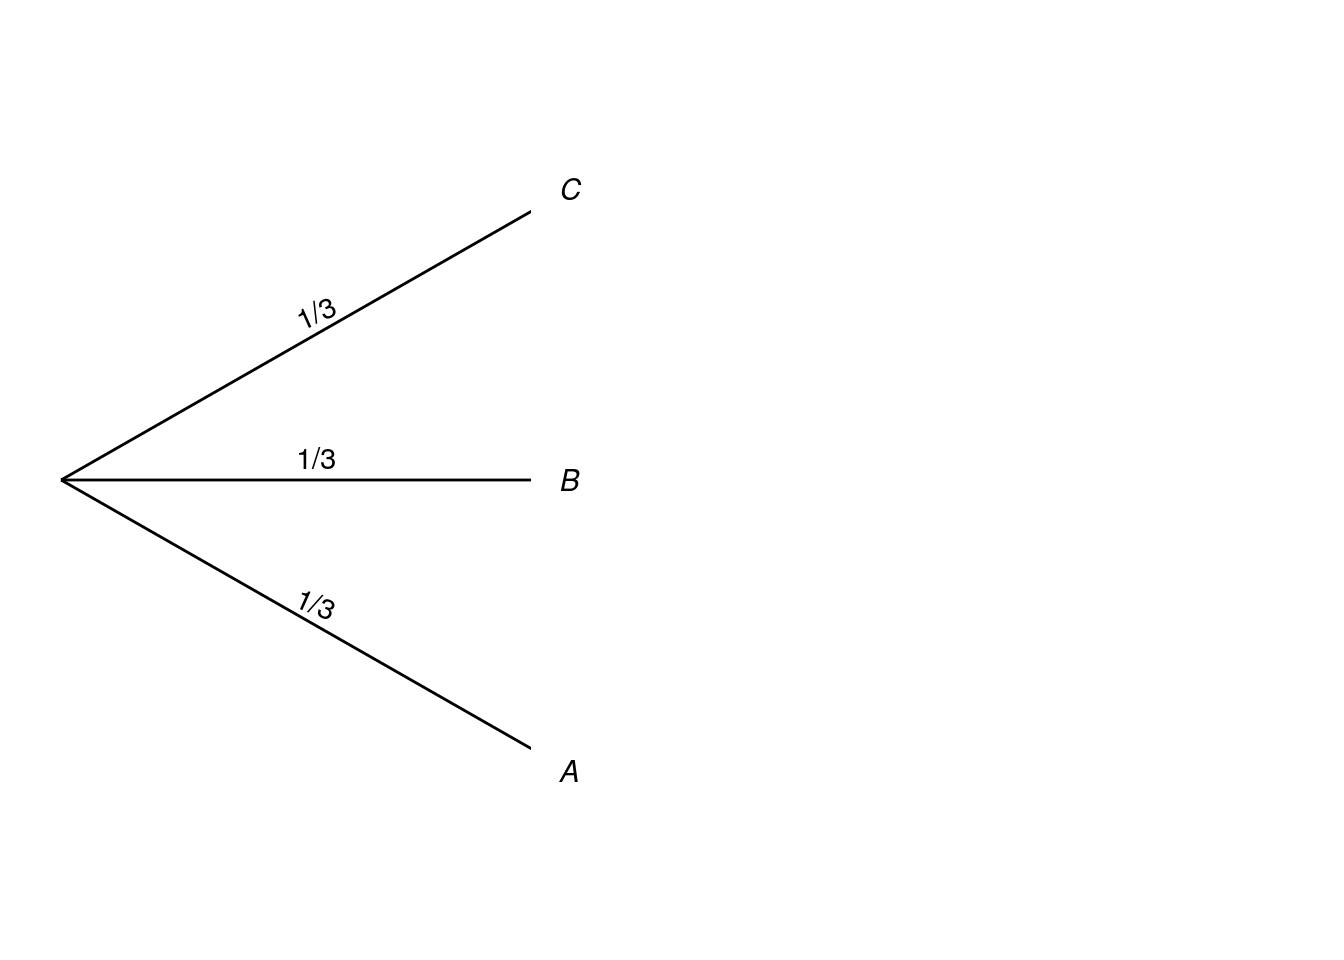
\includegraphics{_main_files/figure-latex/montytree1-1} \caption[First stage of a tree diagram for the Monty Hall problem]{First stage of a tree diagram for the Monty Hall problem}\label{fig:montytree1}
\end{marginfigure}
\begin{marginfigure}
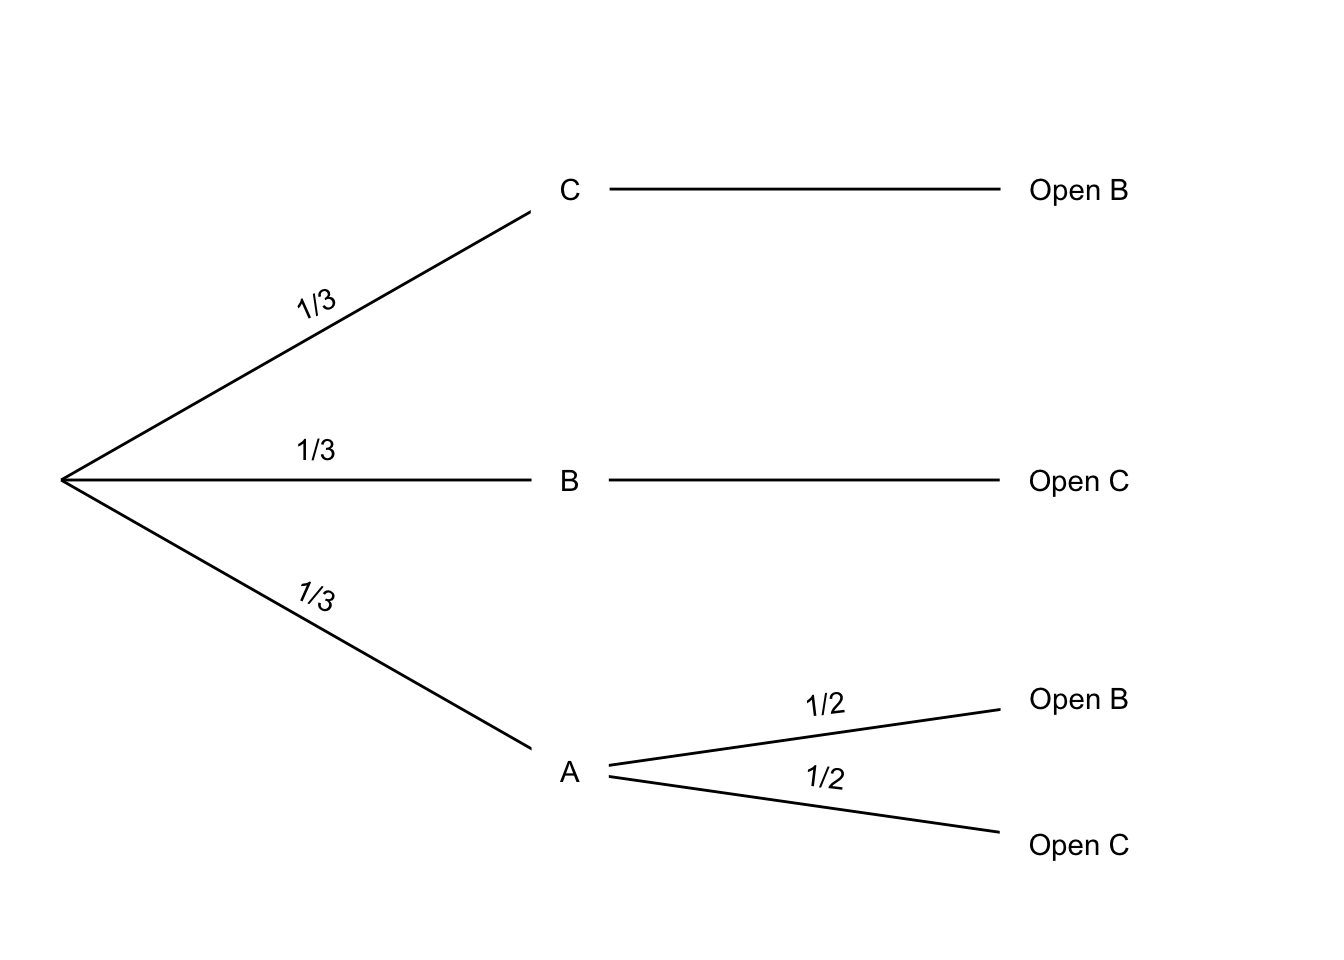
\includegraphics{_main_files/figure-latex/montytree2-1} \caption[Second stage]{Second stage}\label{fig:montytree2}
\end{marginfigure}

\newthought{A} picture helps clarify things. At first the prize could be behind any of the three doors, with equal probability each way. So we draw a tree with three branches, each labeled with a probability of \(1/3\). Figure \ref{fig:montytree1} shows the result.

Now, which door the host opens may depend on where the prize is, i.e.~which branch we're on. If it's behind door C, they won't show you by opening that door. They would have to open door B in this case.

Likewise, if the prize is behind door B, then opening door C is their only option.

Only if the prize is behind door A do they have a choice: open either door B or door C. In that case it's a tossup which door they'll open, so each of those possibilities has a 1/2 chance. Check out Figure \ref{fig:montytree2}.

Now imagine playing the game over and over. A third of the time things will follow the top path; a third of the time they'll follow the middle one; and the remaining third they'll follow one of the two bottom paths.

When things follow the bottom branches, half of those times the host will open door B, and half the time they'll open door C. So one in every six plays will follow the \emph{A-and-Open-B} path. And one in every six plays will follow the \emph{A-and-Open-C} path. See Figure \ref{fig:montytree3}.

Now we can understand what happens when the host opens door C. Usually it's because the prize is behind door B. Sometimes they open door C because the prize is behind door A instead. But that's only a sixth of the time, compared to a third of the time where they open door C because the prize is behind door B.

So when you see the host open door C, you should think it's more likely you're on the middle branch, with the prize behind door B. Switch!

\hypertarget{lessons}{%
\section{Lessons Learned}\label{lessons}}

\newthought{Tree} diagrams are a handy tool for solving probability problems. They also illustrate some central concepts of probability.

Probabilities are numbers assigned to possibilities. In the Monty Hall problem, there are three possibilities for where the prize is: door A, door B, and door C. Each of these possibilities has the same probability: 1/3.

\newthought{Some} possibilities are \textbf{\emph{mutually exclusive}}, meaning only one of them can obtain. The prize can't be behind door A and door B, for example. Here are more examples of mutually exclusive possibilities:

\begin{itemize}
\tightlist
\item
  A coin can land heads or tails, but it can't do both on the same toss.
\item
  A card drawn from a standard deck could be either an ace or a queen, but it can't be both.
\item
  The temperature at noon tomorrow could be 20 degrees, or it could be 25 degrees, but it can't be both.
\end{itemize}

When possibilities are mutually exclusive, their probabilities add up. For example, the initial probability the prize will be behind either door A or door B is \(1/3 + 1/3 = 2/3\). And the probability a card drawn from a standard deck will be either an ace or a queen is \(4/52 + 4/52 = 8/52 = 2/13\).

\newthought{Another} key concept is possibilities that are \textbf{\emph{exhaustive}}. In the Monty Hall problem, the prize has to be behind one of the three doors, so A, B, and C ``exhaust'' all the possibilities. Here are more examples of exhaustive possibilities:

\begin{itemize}
\tightlist
\item
  A card drawn from a standard deck must be either red or black.
\item
  The temperature at noon tomorrow must be either above zero, below zero, or zero.
\end{itemize}

\begin{marginfigure}
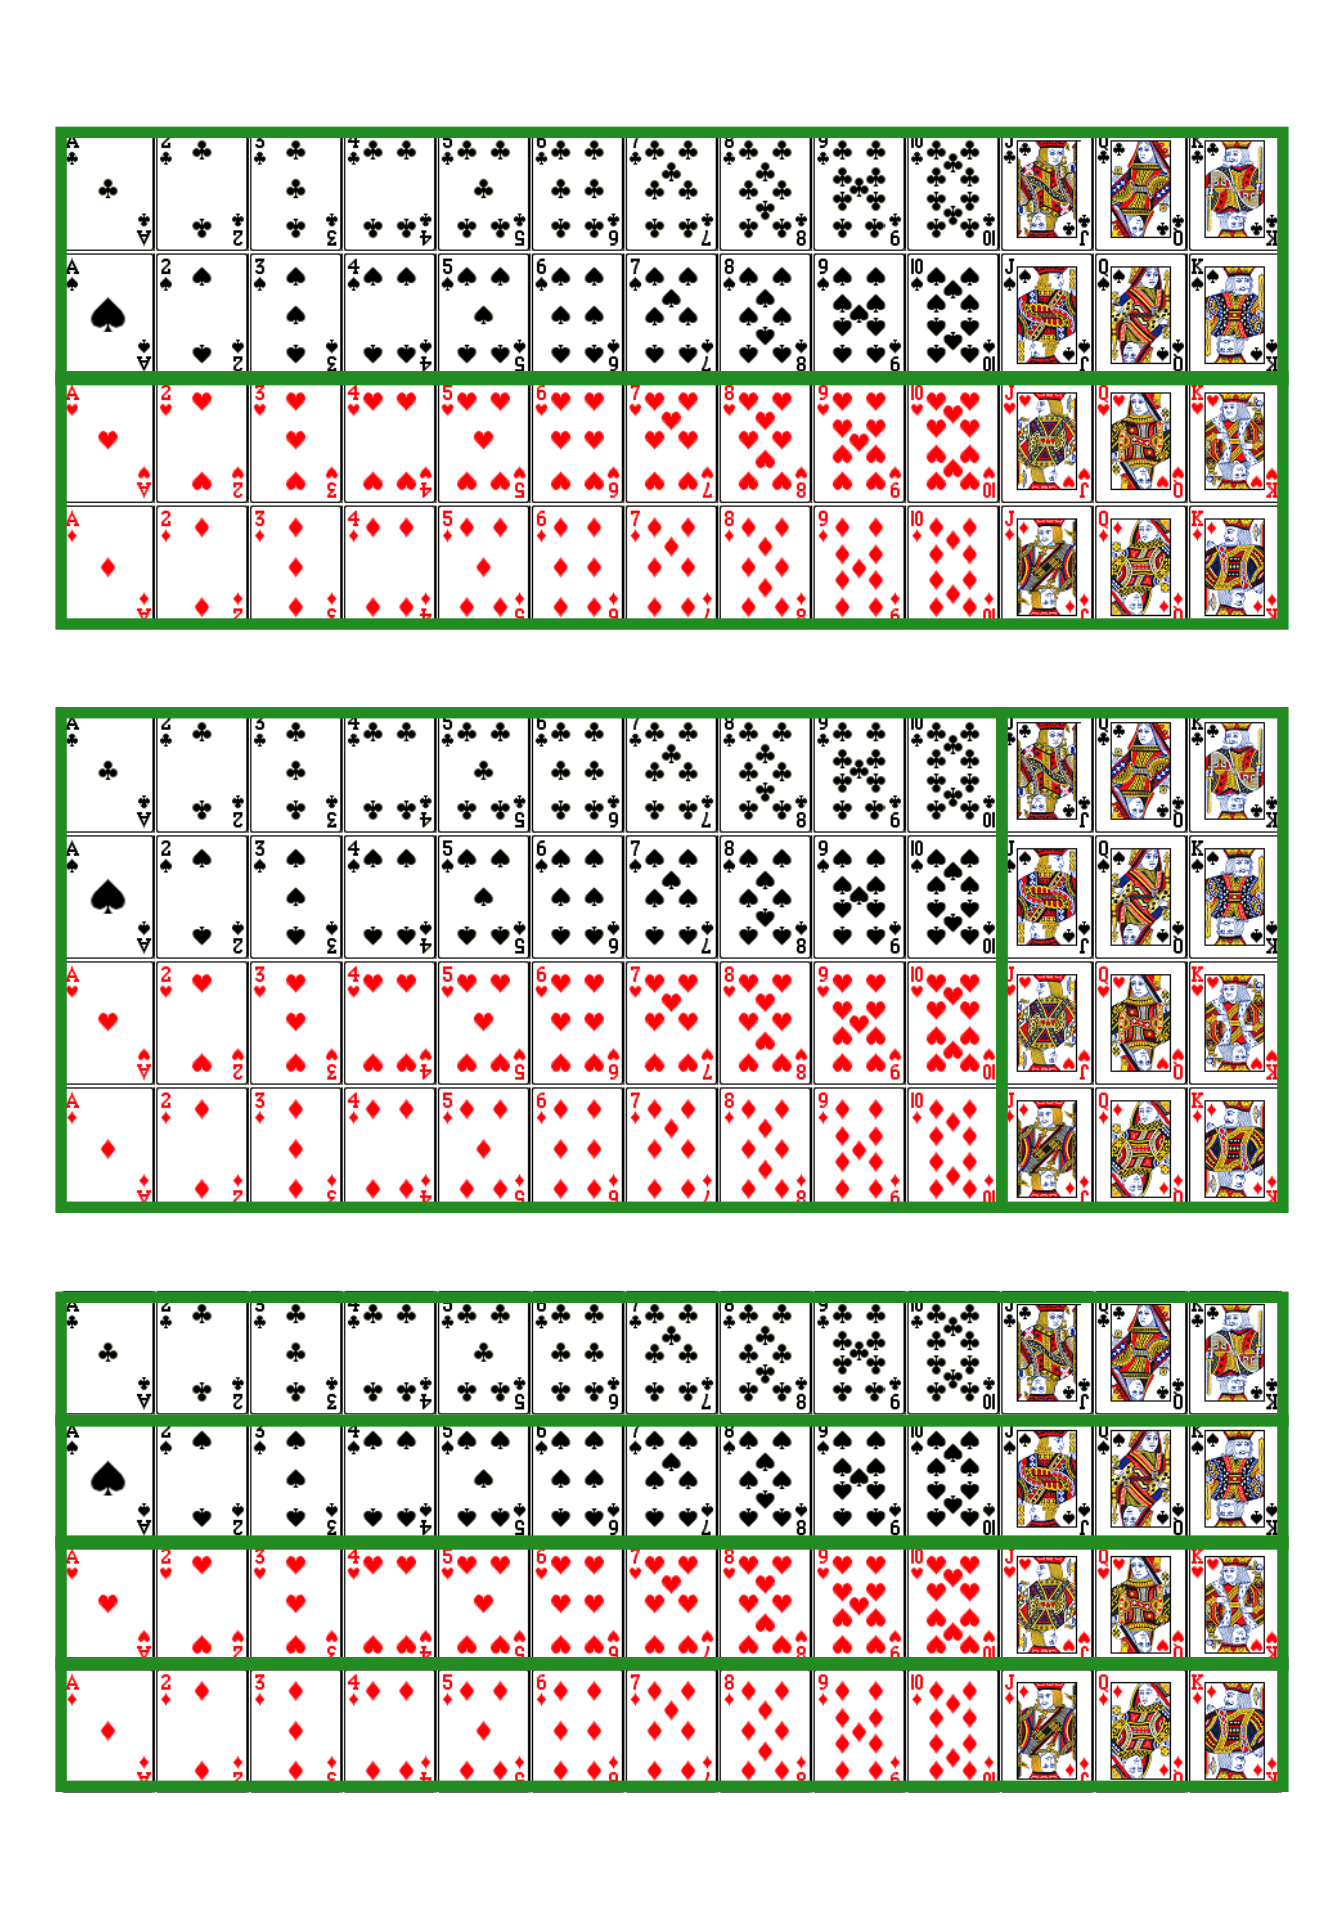
\includegraphics{_main_files/figure-latex/unnamed-chunk-5-1} \caption[Three  partitions for a card drawn from a standard deck]{Three  partitions for a card drawn from a standard deck}\label{fig:unnamed-chunk-5}
\end{marginfigure}

\newthought{In} our tree diagrams, each branch-point always uses a set of possibilities that is \emph{both} exclusive \emph{and} exhaustive. The first split on the three doors covers all the possibilities for where the prize might be, and only one of those possibilities can be the actual location of the prize. Likewise for the second stage of the diagram. On the bottom branch for example, the host must open either door B or door C given the rules, but he will only open one or the other.

When a set of possibilities is both exclusive and exhaustive, it's called a \textbf{\emph{partition}}. A partition ``carves up'' the space of possibilities into distinct, non-overlapping units.

There can be more than one way to partition the space of possibilities. For example, a randomly drawn playing card could be black or red; it could be a face card or not; and it could be any of the four suits (\(\heartsuit\), \(\diamondsuit\), \(\clubsuit\), \(\spadesuit\)).

\newthought{When} possibilities form a partition, their probabilities must add up to 1. Initially, the probability the prize will be behind one of the three doors is \(1/3 + 1/3 + 1/3 = 1\). And the probability that a card drawn from a standard deck at random will be either red or black is \(1/2 + 1/2 = 1\).

In a way, the fundamental principle of probability is that probabilities over a partition must add up to 1.

\newthought{Tree} diagrams follow a few simple rules based on these concepts. The parts of a tree are called \emph{nodes}, \emph{branches}, and \emph{leaves}: see Figure \ref{fig:treeparts}.

\begin{figure}
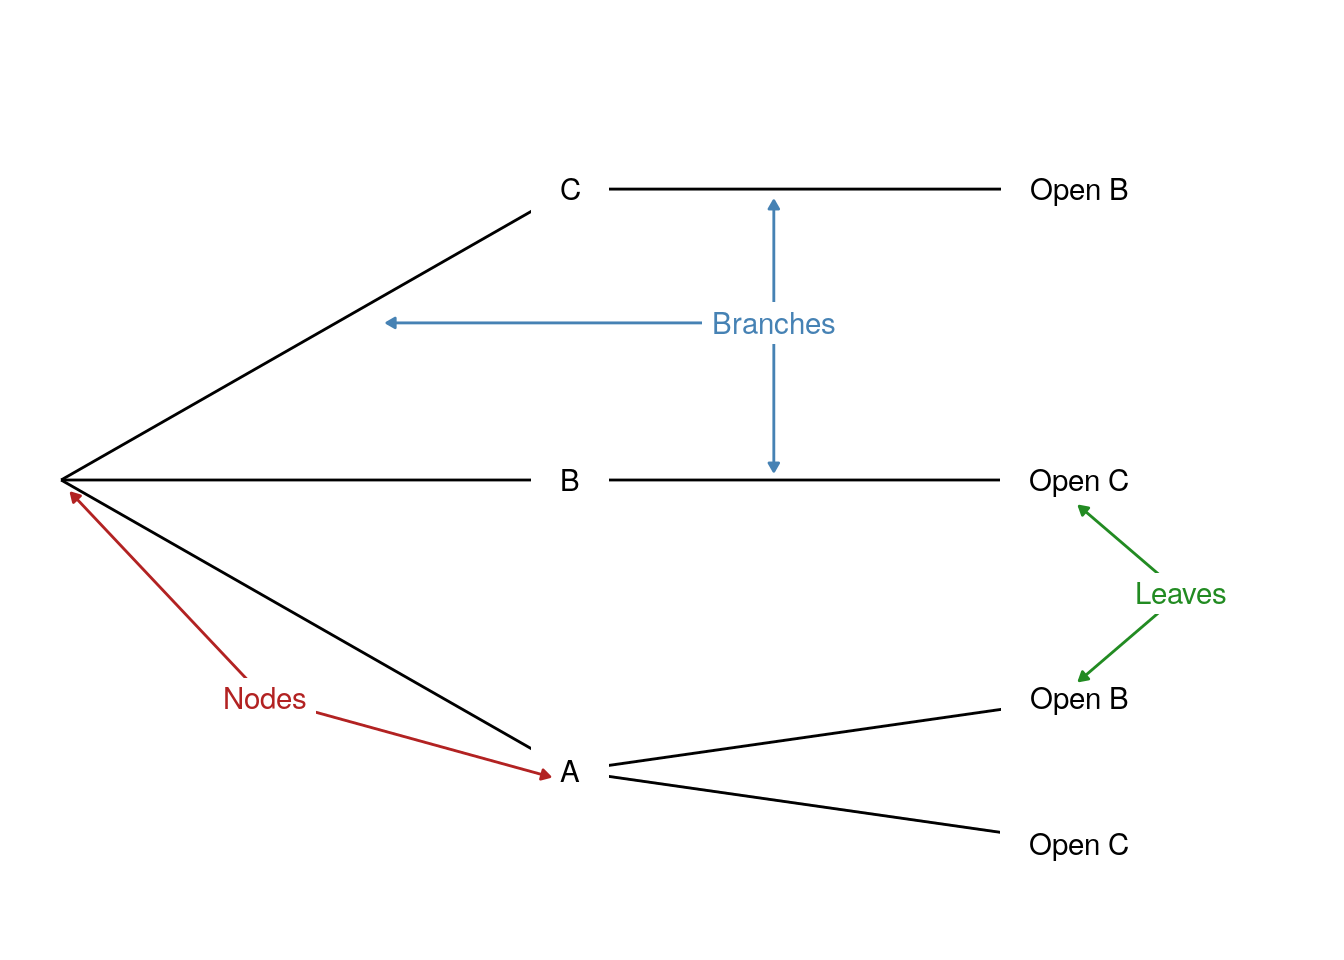
\includegraphics{_main_files/figure-latex/treeparts-1} \caption[The parts of a tree diagram]{The parts of a tree diagram: nodes, branches, and leaves}\label{fig:treeparts}
\end{figure}

The rules for a tree are as follows.

\emph{Rule 1.} Each node must branch into a partition. The subpossibilities that emerge from a node must be mutually exclusive. And they must include every way the possibility from which they emerge could obtain.

\emph{Rule 2.} The probabilities emerging from a node must add to \(1\). If we add up the numbers on the branches immediately coming out of a node, they should add to \(1\).

\emph{Rule 3.} The probability on a branch is \emph{conditional} on the branches leading up to it.

\begin{itemize}
\tightlist
\item
  Consider the bottom path in the Monty Hall problem. The probability the host will open door C is \(1/2\) there because we're assuming the prize is behind door A.
\end{itemize}

\emph{Rule 4.} The probability of a leaf is calculated by multiplying across the branches on the path leading to it. This number represents the probability that all possibilities on that path occur.

Notice, Rule 4 is how we got the final probabilities (the numbers in bold) we used to solve the Monty Hall problem.

\hypertarget{exercises}{%
\section*{Exercises}\label{exercises}}
\addcontentsline{toc}{section}{Exercises}

\begin{enumerate}
\item
  True or false: in the Monty Hall problem, it's essential to the puzzle that the host doesn't want to expose the prize. If they didn't care about giving away the location of the prize, there would be no reason to switch when they open door C.
\item
  In the version of the Monty Hall problem with a hundred doors, after the host opens every door except door 1 (your door) and door 59, the chance the prize is behind door 59 is:

  \begin{enumerate}
  \def\labelenumii{\alph{enumii}.}
  \tightlist
  \item
    1/100
  \item
    1/99
  \item
    1/2
  \item
    99/100
  \end{enumerate}
\item
  Imagine three prisoners, A, B, and C, are condemned to die in the morning. But the king decides to pardon one of them first. He makes his choice at random and communicates it to the guard, who is sworn to secrecy. She can only tell the prisoners that one of them will be released at dawn, she can't say who.

  Prisoner A welcomes the news, as he now has a \(1/3\) chance of survival. Hoping to go even further, he says to the guard, ``I know you can't tell me whether I am condemned or pardoned. But at least one other prisoner must still be condemned, so can you just name one who is?''. The guard tells him that B is still condemned. ``Ok'', says A, ``then it's either me or C who was pardoned. So my chance of survival has gone up to 1/2''.

  Is prisoner A's reasoning correct? Use a probability tree to explain why/why not.
\item
  In a probability tree, each branch point should split into possibilities that are:

  \begin{enumerate}
  \def\labelenumii{\alph{enumii}.}
  \tightlist
  \item
    Mutually exclusive.
  \item
    Exhaustive.
  \item
    Both mutually exclusive and exhaustive.
  \item
    None of the above.
  \end{enumerate}
\item
  Suppose you have two urns. The first has two black marbles and two white marbles. The second has three black marbles and one white marble. You are going to flip a fair coin to select one of the urns at random, and then draw one marble at random. What is the chance you will select a black marble?

  Hint: draw a probability tree and ask yourself, ``if I did this experiment over and over again, how often would I draw a black marble in the long run?''

  \begin{enumerate}
  \def\labelenumii{\alph{enumii}.}
  \tightlist
  \item
    5/8
  \item
    3/8
  \item
    1/2
  \item
    1/4
  \end{enumerate}
\end{enumerate}

\hypertarget{logic}{%
\chapter{Logic}\label{logic}}

\begin{epigraph}
I can win an argument on any topic, against any opponent. People know
this, and steer clear of me at parties. Often, as a sign of their great
respect, they don't even invite me.\\
---Dave Barry
\end{epigraph}

\newthought{Logic} is the study of what follows from what. From the information that Tweety is a bird and all birds are animals, it follows that Tweety is an animal. But things aren't always so certain. Can Tweety fly? Most birds can fly, so probably. But Tweety might be a penguin.

\emph{Deductive} logic is the branch of logic that studies what follows with certainty. \emph{Inductive} logic deals with uncertainty, things that only follow with high probability.

This book is about inductive logic and probability. But we need a few concepts from deductive logic to get started.

\hypertarget{validity-soundness}{%
\section{Validity \& Soundness}\label{validity-soundness}}

\newthought{In} deductive logic we study ``valid'' arguments. An argument is \textbf{\emph{valid}} when the conclusion must be true if the premises are true. Take this example again:

\begin{argument}
Tweety is a bird.\\
All birds are animals.\\
Therefore, Tweety is an animal.
\end{argument}

The first two lines are called the \emph{premises} of the argument. The last line is called the \emph{conclusion}. In this example, the conclusion must be true if the premises are. So the argument is valid.

Here's another example of a valid argument:

\begin{argument}
Tweety is taller than Kwazi.\\
Kwazi is taller than Peso.\\
Therefore, Tweety is taller than Peso.
\end{argument}

The argument is valid because it's just not possible for the premises to be true and the conclusion false.

Here's an example of an \emph{invalid} argument:

\begin{argument}
Tweety is a bird.\\
Most birds can fly.\\
Therefore, Tweety can fly.
\end{argument}

It's not valid because validity requires the conclusion to follow \emph{necessarily}. If there's any way for the the premises to be true yet the conclusion false, the argument doesn't count as valid. And like we said, Tweety might be a penguin.

Valid arguments are interesting because their logic is airtight. If the assumptions of the argument are correct, there's no way to go wrong accepting the conclusion. But what if the assumptions \emph{aren't} correct? Validity isn't everything, we also want our arguments to build on true foundations.

\newthought{We} call an argument \textbf{\emph{sound}} when it is valid \emph{and} all the premises are true:
\[ \mbox{sound = valid + true premises}.\]
For example, here's a sound argument:

\begin{argument}
The author of this book is human.\\
All humans are animals.\\
Therefore, the author of this book is an animal.
\end{argument}

Sound arguments are important because their conclusions are always true. The premises of a sound argument are true by definition. And since it's valid by definition too, that guarantees the conclusion to be true as well.

Yet deductive logic studies validity, not soundness. Why?

Because logicians aren't in the business of determining when the premises of an argument are true. As a logician, I might have no idea who Tweety is, and thus no idea whether Tweety is a bird. I might not even know whether all birds fly, or just some, or even none. That's a job for an ornithologist.

A logician's job is to assess the \emph{logic} of an argument, the connections between its assumptions and its conclusion. So a logician just takes the premises of an argument for granted and asks, how well do those assumptions support the conclusion? That's something you don't need to know any ornithology to study. Or biology, or medicine, or physics, or whatever topic a particular argument concerns.

\newthought{Validity} is a tricky, counterintuitive concept. It's very much a hypothetical notion: it's about whether the conclusion must be true \emph{if} the premises are true. So when we assess an argument's validity, we ignore what we know about the truth of its premises. We pretend they're true even if they aren't. We even have to ignore what we know about the conclusion.

Instead we suspend what we know about the topic, and just imagine the premises to be true. Then we ask: in this hypothetical scenario, is there any way the conclusion could be false? If there is, the argument is invalid. Otherwise, it's valid.

\hypertarget{propositions}{%
\section{Propositions}\label{propositions}}

\newthought{Arguments} are made out of statements, assertions that something is true. In logic we call these statements \textbf{\emph{propositions}}. And we use capital letters of the English alphabet to stand for them. For example, this argument:

\begin{argument}
If Aegon is a tyrant, then Brandon is a wizard.\\
Aegon is a tyrant.\\
Therefore, Brandon is a wizard.
\end{argument}

can be summarized like this:

\begin{argument}
If \(A\), then \(B\).\\
\(A\).\\
Therefore, \(B\).
\end{argument}

\newthought{Not} all sentences are propositions. Some are questions, some are commands, some are expressions of worry. For example:

\begin{itemize}
\tightlist
\item
  What time is it?
\item
  Pass the rooster sauce!
\item
  Uh oh.
\end{itemize}

One way to distinguish propositions from other kinds of sentences is: propositions are capable of being true or false. It wouldn't make sense to respond to someone who asks you what time it is by saying, ``what you just said is false!'' And you wouldn't respond to someone's request to pass the sauce with ``that's true!'' Except maybe as a joke.

\hypertarget{visualizing-propositions}{%
\section{Visualizing Propositions}\label{visualizing-propositions}}

\newthought{We} learned about mutually exclusive propositions in \protect\hyperlink{lessons}{Section} \ref{lessons}. Two propositions are mutually exclusive when one of them being true means the other must be false. For example:

\begin{itemize}
\tightlist
\item
  \(A\): Confucius was born in the 6th Century A.D.
\item
  \(B\): Confucius was born in the 6th Century B.C.
\end{itemize}

There is no way for both of these propositions to be true, and we can visualize this relationship in a diagram (Figure \ref{fig:meprops}).

\begin{marginfigure}
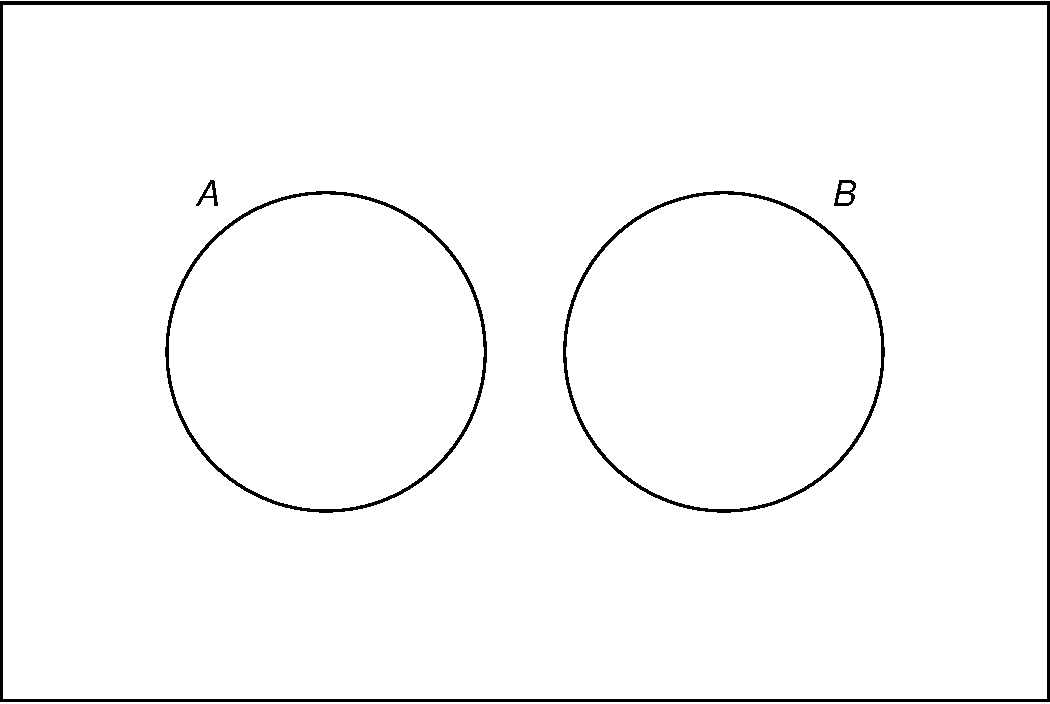
\includegraphics{_main_files/figure-latex/meprops-1} \caption[Mutually exclusive propositions]{Mutually exclusive propositions}\label{fig:meprops}
\end{marginfigure}

Each circle represents a proposition. You can think of it as surrounding the possible situations where the proposition would be true. The circles don't overlap because there is no possible situation where both propositions in this example are true.

In contrast, these two propositions are not mutually exclusive:

\begin{itemize}
\tightlist
\item
  Confucius was born in Asia.
\item
  Confucius was born in the 6th Century B.C.
\end{itemize}

When propositons are not mutually exclusive, we say they are \textbf{\emph{compatible}}. Compatible propositions overlap (Figure \ref{fig:compropositions}). The region where the circles overlap represents the possible scenarios where both propositions are true (the ``\(A \wedge B\) region'').

\begin{marginfigure}
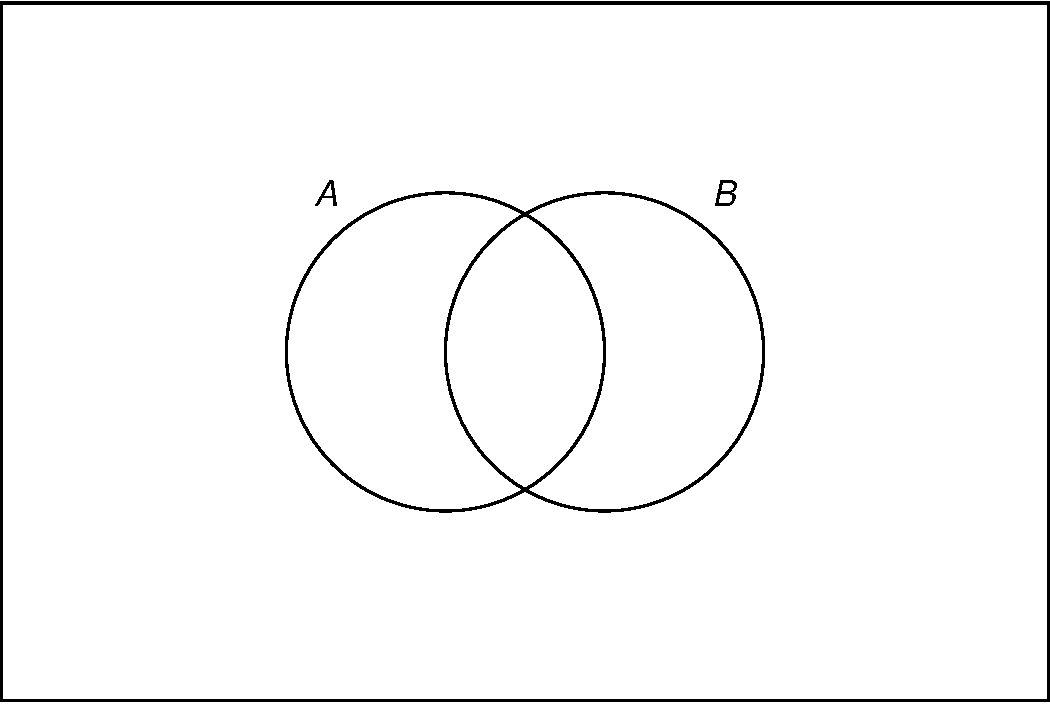
\includegraphics{_main_files/figure-latex/compropositions-1} \caption[Compatible propositions]{Compatible propositions}\label{fig:compropositions}
\end{marginfigure}

These are called \textbf{\emph{Euler diagrams}}, after the mathematician Leonhard Euler (pronounced \emph{oiler}).\footnote{Leonhard Euler lived from \(1707\) to \(1783\). You may have encountered some of his work before if you've worked with logarithms or taken calculus.} You may have seen Venn diagrams before, which are very similar. But in an Euler diagram, the circles don't have to overlap.

\newthought{Sometimes} one circle will even contain another circle entirely. Take this example:

\begin{itemize}
\tightlist
\item
  Confucius was born in Asia.
\item
  Confucius was born somewhere.
\end{itemize}

These propositions aren't just compatible. If the first is true, then the second \emph{must} be true. Imagine an argument with the first proposition as the premise and the second proposition as the conclusion. The argument would be valid:

\begin{argument}
Confucius was born in Asia.\\
Therefore, Confucius was born.
\end{argument}

\begin{marginfigure}
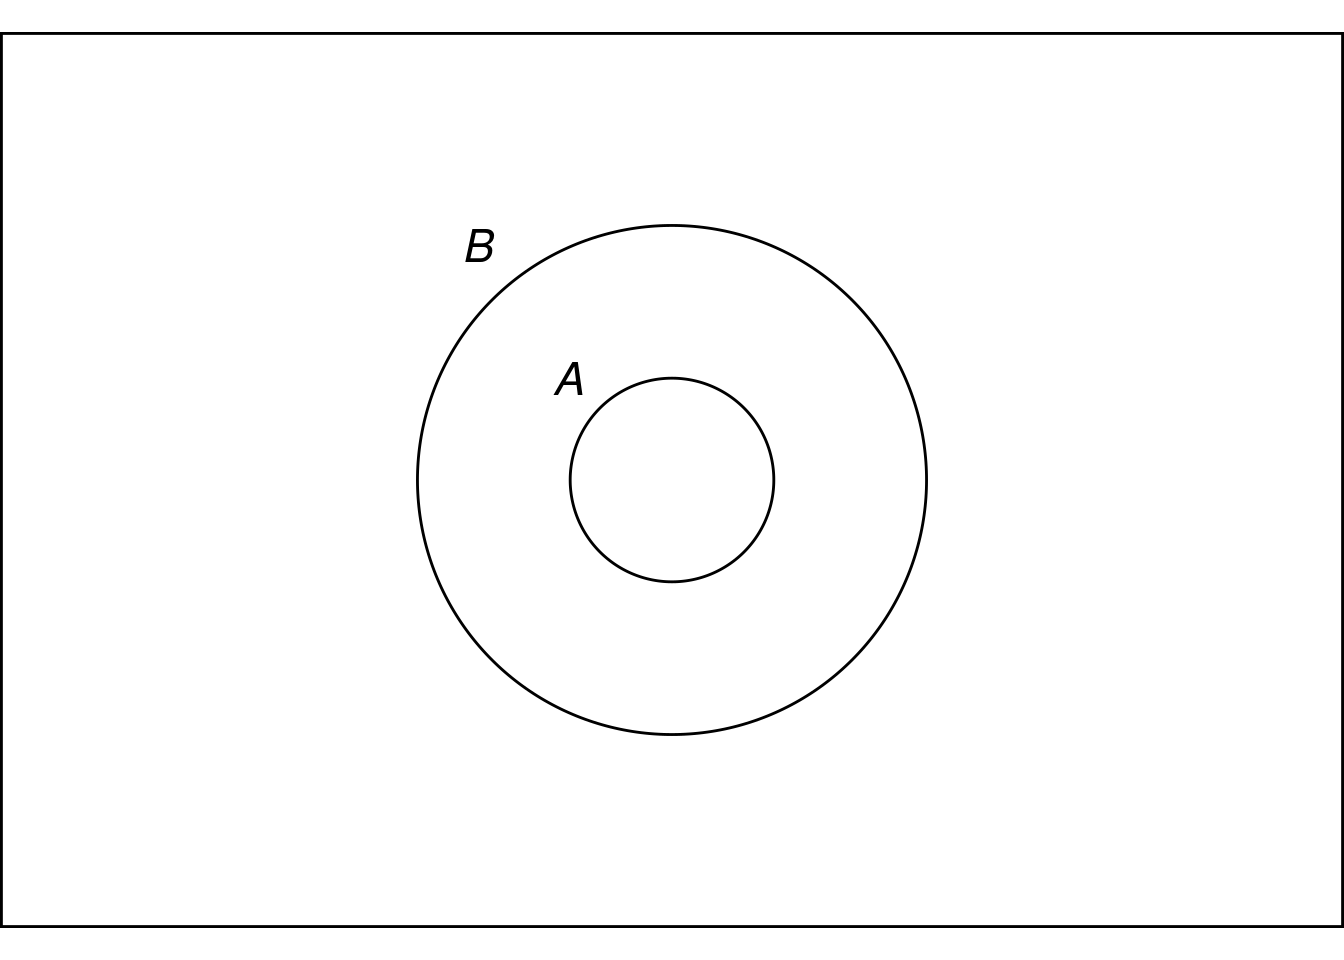
\includegraphics{_main_files/figure-latex/entailment-1} \caption[Logical entailment]{Logical entailment}\label{fig:entailment}
\end{marginfigure}

In this case we say that the first proposition \textbf{\emph{logically entails}} the second. In terms of an Euler diagram, he first circle is contained entirely in the second (Figure \ref{fig:entailment}). Because there is no possible situation where the first proposition is true yet the second false.

What if an argument has multiple premises? For example:

\begin{argument}
Zhuangzi was born in the Chinese province of Anhui.\\
Zhuoru was born in the Chinese city of Beijing.\\
Therefore, both Zhuangzi and Zhuoru were born in China.
\end{argument}

\begin{marginfigure}
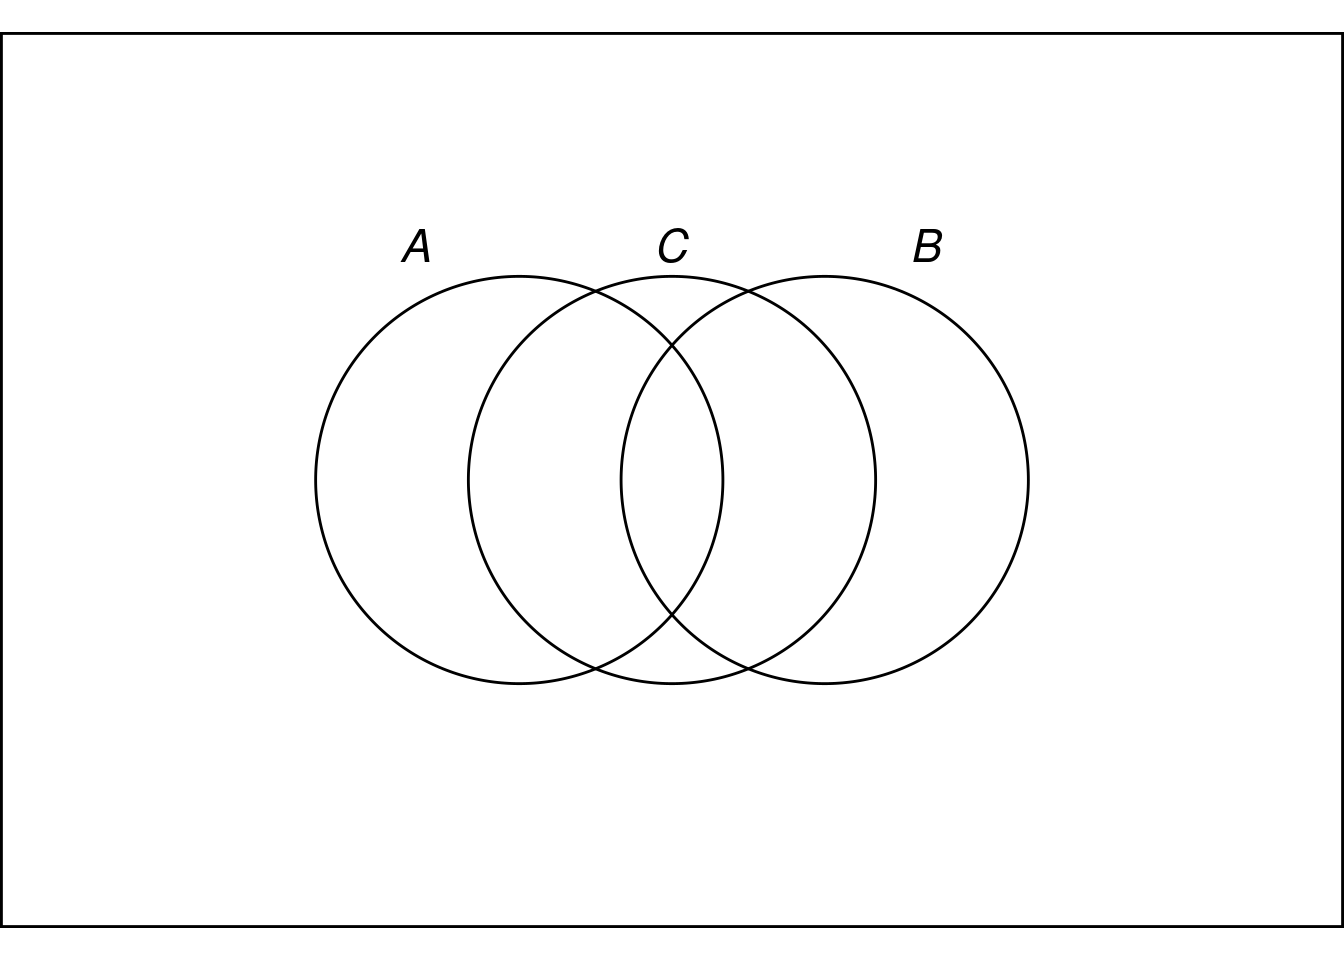
\includegraphics{_main_files/figure-latex/validtwopremises-1} \caption[A valid argument with two premises]{A valid argument with two premises}\label{fig:validtwopremises}
\end{marginfigure}

This argument is valid, and the diagram might look like Figure \ref{fig:validtwopremises}. Notice how the \(A \wedge B\) region lies entirely within the \(C\) circle. This reflects the argument's validity: there is no way for the first two propositions to be true and the last one false.

In contrast, an invalid argument would have a diagram like Figure \ref{fig:invalidtwopremises}. This diagram allows for the possibility that \(A\) and \(B\) are both true yet \(C\) is false; part of the \(A \wedge B\) region falls outside the \(C\) circle.

\begin{marginfigure}
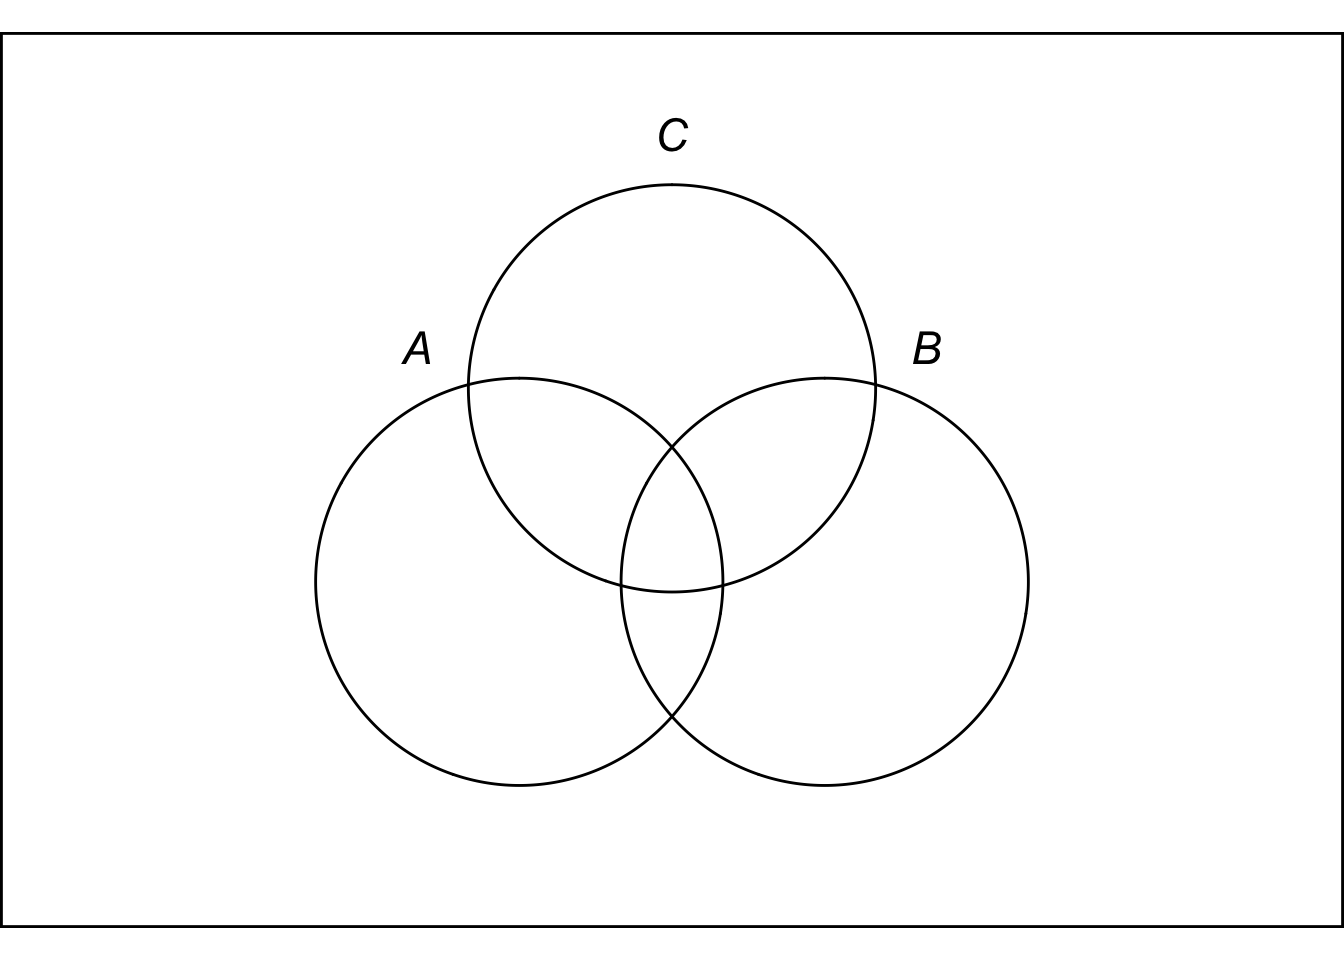
\includegraphics{_main_files/figure-latex/invalidtwopremises-1} \caption[An invalid argument with two premises]{An invalid argument with two premises}\label{fig:invalidtwopremises}
\end{marginfigure}

\hypertarget{strength}{%
\section{Strength}\label{strength}}

\newthought{Inductive} logic studies arguments that aren't necessarily valid, but still ``strong''. A \textbf{\emph{strong}} argument is one where the conclusion is highly probable, if the premises are true. For example:

\begin{argument}
The sun has risen every day so far.\\
Therefore, the sun will rise again tomorrow.
\end{argument}

This argument isn't valid, because it's possible the conclusion is false even though the premise is true. Maybe the sun will explode in the night for some surprising reason. Or maybe the earth's rotation will be stopped by alien forces.

These possibilities aren't very likely, of course. So the argument is strong, even though it's not strictly valid. The premise gives us very good reason to believe the conclusion, just not a 100\% guarantee.

In terms of an Euler diagram then, the premise circle isn't contained entirely within the conclusion circle (Figure \ref{fig:strongarg}). We have to leave some room for the possibility that the premise is true and the conclusion false. But we can still convey that this possibility has only a very slight chance of being true, by making it slim.

\begin{marginfigure}
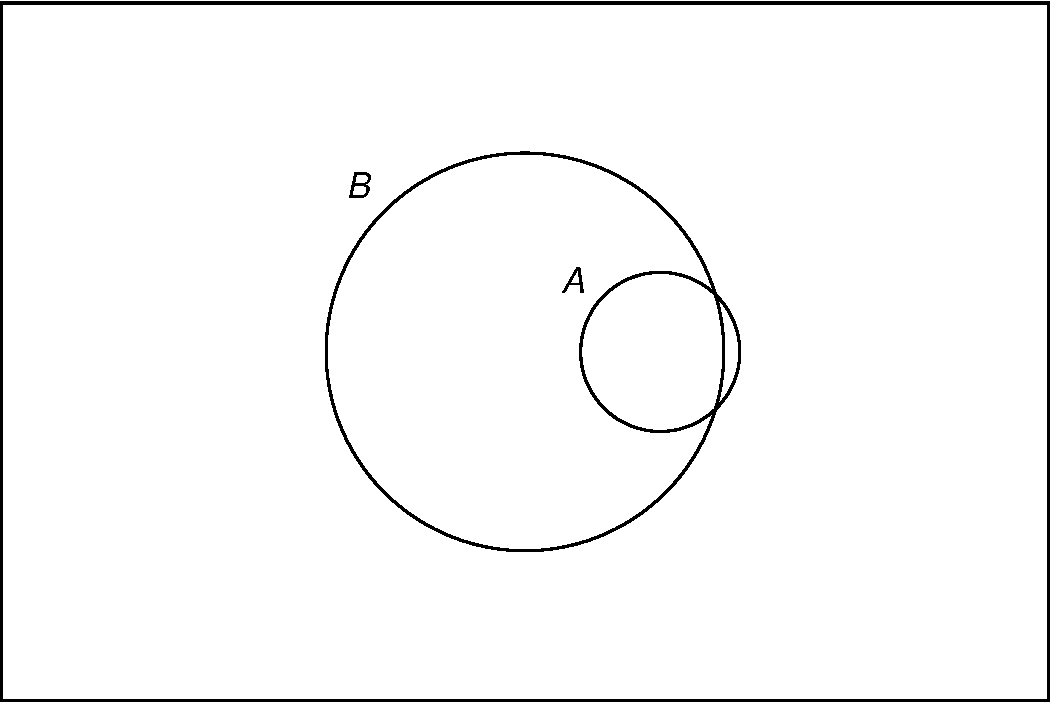
\includegraphics{_main_files/figure-latex/strongarg-1} \caption[A strong argument with premise $A$ and conclusion $B$]{A strong argument with premise $A$ and conclusion $B$}\label{fig:strongarg}
\end{marginfigure}



\begin{marginfigure}
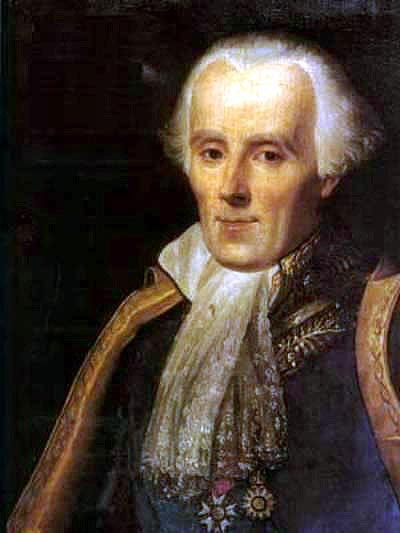
\includegraphics[width=1.33in]{img/laplace} \caption[Pierre Simone Laplace (1749--1827) developed \href{https://bit.ly/2mU9WgW}{a formula} for calculating the probability the sun will rise tomorrow. We'll learn how to do similar calculations in the coming chapters.]{Pierre Simone Laplace (1749--1827) developed \href{https://bit.ly/2mU9WgW}{a formula} for calculating the probability the sun will rise tomorrow. We'll learn how to do similar calculations in the coming chapters.}\label{fig:laplace}
\end{marginfigure}

We could also label the \emph{\(A\)-but-not-\(B\)} region with a small number, if we knew exactly how unlikely this possibility was.

\newthought{Strength} comes in degrees. An argument's premises can make the conclusion somewhat likely, very likely, almost certain, or perfectly certain. So arguments range from weak, to somewhat strong, to very strong, etc.

Strength differs from validity here, since validity is all-or-nothing. If there is any possible way for the premises to be true and the conclusion false, the argument is invalid---no matter how remote or bizarre that possibility is.

Notice though, valid arguments are strong by definition. Since it's impossible for a valid argument's conclusion to be false if the premises are true, the premises make the conclusion 100\% probable. A valid argument is the strongest possible argument.

\hypertarget{indargs}{%
\section{Forms of Inductive Argument}\label{indargs}}

\newthought{What} kinds of strong arguments are there, and how strong are they? That's what the rest of this book is about, in a way. But we can start by identifying some common forms of inductive argument right now.

\newthought{Generalizing} from observed instances is one extremely common form of argument:

\begin{argument}
Every raven I have ever seen has been black.\\
Therefore, all ravens are black.
\end{argument}

Arguments of this kind are usually stronger the more instances you observe. If you've only ever seen two ravens, this argument won't be very compelling. But if you've seen thousands, then it's much stronger.

It also helps to observe different kinds of instances. If you've only observed ravens in your city or town, then even the thousands you've seen won't count for much. Maybe the raven population in your area is unusual, and ravens on the other side of the world are all different colours.

\newthought{Going} in the opposite direction, we can use what we know about a general population to draw conclusions about particular instances. We saw an example of this earlier:

\begin{argument}
Most birds can fly.\\
Tweety is a bird.\\
Therefore, Tweety can fly.
\end{argument}

Again, the strength of the inference depends on the details. If ``most birds'' means \(99\%\), the argument is quite strong. If ``most'' only means \(80\%\), then it's not so strong. (Usually ``most'' just means more than \(50\%\).)

It also helps to know that Tweety is similar to the birds that can fly, and different from the ones that can't. If we know that Tweety is small and has feathers, that makes the argument stronger. If instead we know that Tweety is large, and coloured black and white, that makes the argument weaker. It suggests Tweety is a penguin.

\newthought{Inference} to the best explanation is another common form of argument, quite different from the previous two. Here's an example:

\begin{argument}
My car won't start and the gas gauge reads `empty'.\\
Therefore, my car is out of gas.
\end{argument}

An empty tank would explain the sytmptoms described in the premise, so the premise makes the conclusion plausible. There could be other possible explanations, of course. Maybe the engine and the gas gauge both just happened to break at the same time. But that would be quite a coincidence, so this explanation isn't as good.

What makes one explanation better than another? That turns out to be a very hard question, and there is no generally accepted answer. We'll come back to this issue later, once we have a better grip on the basics of probability.

\hypertarget{exercises-1}{%
\section*{Exercises}\label{exercises-1}}
\addcontentsline{toc}{section}{Exercises}

\begin{enumerate}
\item
  For each of the following arguments, say whether it is valid or invalid.

  \begin{enumerate}
  \def\labelenumii{\alph{enumii}.}
  \item
    \begin{argument}
    All cats have whiskers.\\
    Simba has whiskers.\\
    Therefore, Simba is a cat.
    \end{argument}
  \item
    \begin{argument}
    Ada Lovelace wrote the world's first computer program.\\
    Ada Lovelace was Lord Byron's daughter.\\
    Therefore, the first computer program was written by Lord Byron's
    daughter.
    \end{argument}
  \item
    \begin{argument}
    All Canadian residents are Russian citizens.\\
    Vladimir Putin is a Canadian resident.\\
    Therefore, Vladimir Putin is a Russian citizen.
    \end{argument}
  \item
    \begin{argument}
    Manitoba is located in either Saskatchewan, Ontario, or Quebec.\\
    Manitoba is not located in Saskatchewan.\\
    Manitoba is not located in Ontario.\\
    Therefore, Manitoba is located in Quebec.
    \end{argument}
  \item
    \begin{argument}
    If snow is black then pigs can fly.\\
    Snow is not black.\\
    Therefore, pigs cannot fly.
    \end{argument}
  \item
    \begin{argument}
    Either the moon is made of green cheese or pigs can fly.\\
    Pigs can't fly.\\
    Therefore the moon is made of green cheese.\\
    \end{argument}
  \end{enumerate}
\item
  For each pair of propositions, say whether they are mutually exclusive or compatible.

  \begin{enumerate}
  \def\labelenumii{\alph{enumii}.}
  \item
    Regarding the roll of an ordinary die:

    \begin{itemize}
    \tightlist
    \item
      The die will land on an even number.
    \item
      The die will land either \(4\) or \(5\).
    \end{itemize}
  \item
    Regarding the unemployment rate in your country tomorrow:

    \begin{itemize}
    \tightlist
    \item
      The unemployment rate will be at least \(5\%\).
    \item
      The unemployment rate will be exactly \(5\%\).
    \end{itemize}
  \item
    Regarding a party tomorrow:

    \begin{itemize}
    \tightlist
    \item
      Ani will be there and so will her sister PJ.
    \item
      PJ will not be there.
    \end{itemize}
  \end{enumerate}
\item
  True or false? If \(A\) and \(B\) are mutually exclusive, and \(B\) and \(C\) are also mutually exclusive, then \(A\) and \(C\) are mutually exclusive.
\item
  True or false? If \(A\) and \(B\) are mutually exclusive, then \(A\) logically entails that \(B\) is false.
\item
  True or false? It is possible for \(A\) to logically entail \(B\) even though the reverse does not hold (i.e.~even though \(B\) does not logically entail \(A\)).
\item
  Create your own example of each of the three types of inductive argument described in this chapter:

  \begin{enumerate}
  \def\labelenumii{\alph{enumii}.}
  \tightlist
  \item
    Generalizing from Observed Instances
  \item
    Inferring an Instance from a Generalization
  \item
    Inference to the Best Explanation
  \end{enumerate}
\end{enumerate}

\hypertarget{truth-tables}{%
\chapter{Truth Tables}\label{truth-tables}}

\newthought{In} this chapter we'll introduce the last few concepts we need from deductive logic, and we'll learn a useful technique in the process: truth tables.

\hypertarget{connectives}{%
\section{Connectives}\label{connectives}}

\newthought{Complex} propositions can be built up out of other, simpler propositions:

\begin{itemize}
\tightlist
\item
  Aegon is a tyrant \textbf{and} Brandon is a wizard.
\item
  \textbf{Either} Aegon is a tyrant \textbf{or} Brandon is a wizard.
\item
  \textbf{It's not true that} Aegon is a tyrant.
\end{itemize}

\begin{marginfigure}
Notice, we call \emph{it's not true that} a connective even though it
doesn't actually connect two propositions together.
\end{marginfigure}

Here we've used two simple propositions to build up longer, more complex ones using the terms \emph{and}, \emph{either/or}, and \emph{it's not true that}. Such terms are called \textbf{\emph{connectives}}.

The three connectives just listed are the only ones we'll need in this book. Each has a name and a shorthand symbol:

\begin{longtable}[]{@{}llll@{}}
\toprule
Name & English & Symbol & Example\tabularnewline
\midrule
\endhead
conjunction & and & \(\wedge\) & \(A \wedge B\)\tabularnewline
disjunction & either/or & \(\vee\) & \(A \vee B\)\tabularnewline
negation & it's not true that & \(\neg\) & \(\neg A\)\tabularnewline
\bottomrule
\end{longtable}

Here are some more examples of complex propositions:

\begin{itemize}
\tightlist
\item
  \(F \wedge \neg G\): Florida is warm and Geneva is not.
\item
  \(\neg J \vee \neg K\): Either Jing won't come to the party or Kamal won't come.
\end{itemize}

\newthought{Sometimes} we also need parentheses, to avoid ambiguity. Consider an example from arithmetic:
\[ 4 \div 2 \times 2 = 1. \]
Is this equation true? That depends on what you mean. Does the division operation come first, or the multiplication? So we use parentheses to clarify: \(4 \div (2 \times 2) = 1\), but \((4 \div 2) \times 2 = 4\).

In logic we use parentheses to prevent ambiguity similarly. Consider:
\[ A \vee B \wedge C. \]
This proposition is ambiguous, it has two interpretations. In English we can distinguish them with a comma:

\begin{itemize}
\tightlist
\item
  Either Aegon is a tyrant or Brandon is a wizard, and Cerci is the queen.
\item
  Either Aegon is a tyrant, or Brandon is a wizard and Cerci is the queen.
\end{itemize}

Notice how these statements make different claims. The first takes a definite stand on Cerci: she is the queen. It only leaves open the question whether Aegon is a tyrant or Brandon is a wizard. Whereas the second statement takes no definite stand on any of our three characters. Maybe Aegon is a tyrant, maybe not. Maybe Brandon is a wizard and Cerci is the queen, maybe not.

In logic we use parentheses to clarify which interpretation we mean:

\begin{itemize}
\tightlist
\item
  \((A \vee B) \wedge C\).
\item
  \(A \vee (B \wedge C)\).
\end{itemize}

Notice how the first statement is primarily an \(\wedge\) statement. It uses \(\wedge\) to combine the simpler statements \(C\) and \(A \vee B\) together. Whereas the second statement is primarily a \(\vee\) statement. It uses \(\vee\) to combine \(A\) with \(B \wedge C\).

We call the last connective used to build up the statement the \textbf{\emph{main connective}}.

\begin{itemize}
\tightlist
\item
  \((A \vee B) \wedge C\): main connective is \(\wedge\).
\item
  \(A \vee (B \wedge C)\): main connective is \(\vee\).
\end{itemize}

Two more examples:

\begin{itemize}
\tightlist
\item
  \(\neg (A \vee B)\): main connective is \(\neg\).
\item
  \(\neg A \vee B\): main connective is \(\vee\).
\end{itemize}

Technically, the last example should have parentheses to prevent ambiguity, like so: \((\neg A) \vee B\). But things get cluttered and hard to read if we add parentheses around every negation. So we have a special understanding for \(\neg\) in order to keep things tidy.

\begin{marginfigure}
This special understanding for \(\mathbin{\sim}\) mirrors the one for
minus signs in arithmetic.
\end{marginfigure}

\begin{info}
The negation symbol \(\mathbin{\sim}\) only applies to the proposition
immediately following it.
\end{info}

So in the proposition \(\neg A \vee B\), the \(\neg\) only applies to \(A\). And in \(\neg (A \wedge B) \vee C\), it only applies to \(A \wedge B\).

\hypertarget{truth-tables-1}{%
\section{Truth Tables}\label{truth-tables-1}}

\newthought{The} truth of a complex proposition built using our three connectives depends on the truth of its components. For example, \(\neg A\) is false if \(A\) is true, and it's true if \(A\) is false:

\begin{longtable}[]{@{}cc@{}}
\caption{\label{tab:unnamed-chunk-29}Truth table for \(\neg\)}\tabularnewline
\toprule
\(A\) & \(\neg A\)\tabularnewline
\midrule
\endfirsthead
\toprule
\(A\) & \(\neg A\)\tabularnewline
\midrule
\endhead
T & F\tabularnewline
F & T\tabularnewline
\bottomrule
\end{longtable}

Slightly more complicated is the rule for \(\&\):

\begin{longtable}[]{@{}ccc@{}}
\caption{\label{tab:unnamed-chunk-30}Truth table for \(\wedge\)}\tabularnewline
\toprule
\(A\) & \(B\) & \(A \wedge B\)\tabularnewline
\midrule
\endfirsthead
\toprule
\(A\) & \(B\) & \(A \wedge B\)\tabularnewline
\midrule
\endhead
T & T & T\tabularnewline
T & F & F\tabularnewline
F & T & F\tabularnewline
F & F & F\tabularnewline
\bottomrule
\end{longtable}

There are four rows now because \(\&\) combines two propositions \(A\) and \(B\) together to make the more complex proposition \(A \& B\). Since each of those propositions could be either true or false, there are \(2 \times 2 = 4\) possible situations to consider.

Notice that in only one of these situations is \(A \& B\) true, namely the first row where both \(A\) and \(B\) are true.

The truth table for \(\vee\) (``either/or'') is a little more surprising:

\begin{longtable}[]{@{}ccc@{}}
\caption{\label{tab:unnamed-chunk-31}Truth table for \(\vee\)}\tabularnewline
\toprule
\(A\) & \(B\) & \(A \vee B\)\tabularnewline
\midrule
\endfirsthead
\toprule
\(A\) & \(B\) & \(A \vee B\)\tabularnewline
\midrule
\endhead
T & T & T\tabularnewline
T & F & T\tabularnewline
F & T & T\tabularnewline
F & F & F\tabularnewline
\bottomrule
\end{longtable}

Now the complex proposition is always true, except in one case: the last row where \(A\) and \(B\) are both false. It makes sense that \(A \vee B\) is false when both sides are false. But why is it true when both sides are true? Doesn't ``Either \(A\) or \(B\)'' mean that \emph{just one} of these is true?

Sometimes it does have that meaning. But sometimes it means ``Either A or B, \emph{or both}''. Consider this exchange:

\begin{quote}
X: What are you doing tomorrow night?\\
Y: I'm either going to a friend's house or out to a club. I might even do both, if there's time.
\end{quote}

Person Y isn't necessarily changing their mind here. They could just be clarifying: they're doing at least one of these things, possibly even both of them.

Although it's common to use ``either/or'' in English to mean \emph{just} one or the other, in logic we use the more permissive reading. So \(A \vee B\) means \emph{either \(A\), or \(B\), or both}.

We can always convey the stricter way of meaning ``either/or'' with a more complex construction:
\[(A \vee B) \wedge \neg (A \wedge B).\]
That says:
\[ \mbox{Either $A$ or $B$ is true, and it's not the case that both $A$ and $B$ are true}.\]
Which is just a very explicit way of saying: either one or the other, but not both.

We can even verify that the complex construction captures the meaning we want using a truth table. We start with an empty table, where the header lists all the formulas we use to build up to the final, complex one we're interested in:

\begin{longtable}[]{@{}cccccc@{}}
\toprule
\(A\) & \(B\) & \(A \vee B\) & \(A \& B\) & \(\neg(A \wedge B\)) & \((A \vee B) \wedge \neg (A \wedge B)\)\tabularnewline
\midrule
\endhead
\(\;\) & & & & &\tabularnewline
\(\;\) & & & & &\tabularnewline
\(\;\) & & & & &\tabularnewline
\(\;\) & & & & &\tabularnewline
\bottomrule
\end{longtable}

Then we fill in the possible truth values for the simplest propositions, \(A\) and \(B\):

\begin{longtable}[]{@{}cccccc@{}}
\toprule
\(A\) & \(B\) & \(A \vee B\) & \(A \& B\) & \(\neg(A \wedge B\)) & \((A \vee B) \wedge \neg (A \wedge B)\)\tabularnewline
\midrule
\endhead
T & T & & & &\tabularnewline
T & F & & & &\tabularnewline
F & T & & & &\tabularnewline
F & F & & & &\tabularnewline
\bottomrule
\end{longtable}

Next we consult the truth tables above for \(\&\) and \(\vee\) to fill in the columns at the next level of complexity:

\begin{longtable}[]{@{}cccccc@{}}
\toprule
\(A\) & \(B\) & \(A \vee B\) & \(A \& B\) & \(\neg(A \wedge B\)) & \((A \vee B) \wedge \neg (A \wedge B)\)\tabularnewline
\midrule
\endhead
T & T & T & T & &\tabularnewline
T & F & T & F & &\tabularnewline
F & T & T & F & &\tabularnewline
F & F & F & F & &\tabularnewline
\bottomrule
\end{longtable}

Then move up to the next level of complexity. To fill in the column for \(\neg(A \wedge B)\), we consult the column for \(A \wedge B\) and apply the rules from the table for \(\neg\):

\begin{longtable}[]{@{}cccccc@{}}
\toprule
\(A\) & \(B\) & \(A \vee B\) & \(A \& B\) & \(\neg(A \wedge B\)) & \((A \vee B) \wedge \neg (A \wedge B)\)\tabularnewline
\midrule
\endhead
T & T & T & T & F &\tabularnewline
T & F & T & F & T &\tabularnewline
F & T & T & F & T &\tabularnewline
F & F & F & F & T &\tabularnewline
\bottomrule
\end{longtable}

Finally, we consult the columns for \(A \vee B\) and \(\neg(A \wedge B)\), and the table for \(\&\), to fill in the column for \((A \vee B) \wedge \neg(A \& B)\):

\begin{longtable}[]{@{}cccccc@{}}
\toprule
\(A\) & \(B\) & \(A \vee B\) & \(A \& B\) & \(\neg(A \wedge B\)) & \((A \vee B) \wedge \neg (A \wedge B)\)\tabularnewline
\midrule
\endhead
T & T & T & T & F & F\tabularnewline
T & F & T & F & T & T\tabularnewline
F & T & T & F & T & T\tabularnewline
F & F & F & F & T & F\tabularnewline
\bottomrule
\end{longtable}

Complex constructions like this are difficult at first, but don't worry. With practice they quickly become routine.

\hypertarget{logical-truths-contradictions}{%
\section{Logical Truths \& Contradictions}\label{logical-truths-contradictions}}

\newthought{Some} propositions come out true in every row of the truth table. Consider \(A \vee \neg A\) for example:

\begin{longtable}[]{@{}ccc@{}}
\toprule
\(A\) & \(\neg A\) & \(A \vee \neg A\)\tabularnewline
\midrule
\endhead
T & F & T\tabularnewline
F & T & T\tabularnewline
\bottomrule
\end{longtable}

Such propositions are especially interesting because they \emph{must} be true. Their truth is guaranteed, just as a matter of logic. So we call them \textbf{\emph{logical truths}}.

The other side of this coin is propositions that are false in every row of the truth table, like \(A \wedge \neg A\):

\begin{longtable}[]{@{}ccc@{}}
\toprule
\(A\) & \(\neg A\) & \(A \wedge \neg A\)\tabularnewline
\midrule
\endhead
T & F & F\tabularnewline
F & T & F\tabularnewline
\bottomrule
\end{longtable}

These propositions are called \textbf{\emph{contradictions}}.

Notice that the negation of a contradiction is a logical truth. For example, consider the truth table for \(\neg (A \wedge \neg A)\):

\begin{longtable}[]{@{}cccc@{}}
\toprule
\(A\) & \(\neg A\) & \(A \wedge \neg A\) & \(\neg (A \wedge \neg A)\)\tabularnewline
\midrule
\endhead
T & F & F & T\tabularnewline
F & T & F & T\tabularnewline
\bottomrule
\end{longtable}

\hypertarget{mutual-exclusivity-truth-tables}{%
\section{Mutual Exclusivity \& Truth Tables}\label{mutual-exclusivity-truth-tables}}

\newthought{Truth} tables can be used to establish that two propositions are mutually exclusive. A very simple example is the propositions \(A\) and \(\neg A\):

\begin{longtable}[]{@{}cc@{}}
\toprule
\(A\) & \(\neg A\)\tabularnewline
\midrule
\endhead
T & F\tabularnewline
F & T\tabularnewline
\bottomrule
\end{longtable}

There is no row in the table where both propositions are true. And if two propositions can't both be true, they are mutually exclusive by definition.

A slightly more complex example is the propositions \(A \vee B\) and \(\neg A \wedge \neg B\):

\begin{longtable}[]{@{}cccccc@{}}
\toprule
\(A\) & \(B\) & \(\neg A\) & \(\neg B\) & \(A \vee B\) & \(\neg A \wedge \neg B\)\tabularnewline
\midrule
\endhead
T & T & F & F & T & F\tabularnewline
T & F & F & T & T & F\tabularnewline
F & T & T & F & T & F\tabularnewline
F & F & T & T & F & T\tabularnewline
\bottomrule
\end{longtable}

Again there's no row where \(A \vee B\) and \(\neg A \wedge \neg B\) are both true. So they are mutually exclusive.

\hypertarget{entailment-equivalence}{%
\section{Entailment \& Equivalence}\label{entailment-equivalence}}

\newthought{Truth} tables can also be used to establish that an argument is valid. Here's a very simple example:

\begin{quote}
\(A \wedge B\).\\
Therefore, \(A\).
\end{quote}

Obviously it's not possible for the premise to be true and the conclusion false, so the argument is valid (if a bit silly). Accordingly, there is no line of the truth table where \(A \wedge B\) comes out true, yet \(A\) comes out false:

\begin{longtable}[]{@{}ccc@{}}
\toprule
\(A\) & \(B\) & \(A \wedge B\)\tabularnewline
\midrule
\endhead
T & T & T\tabularnewline
T & F & F\tabularnewline
F & T & F\tabularnewline
F & F & F\tabularnewline
\bottomrule
\end{longtable}

The only line where \(A \wedge B\) comes out true is the first one. And on that line \(A\) is true too. So the argument from \(A \wedge B\) to \(A\) is valid.

One more example:

\begin{quote}
\(A \vee B\).\\
\(\neg A\).\\
Therefore, \(B\).
\end{quote}

This argument is valid because the first premise says that at least one of the two propositions \(A\) and \(B\) must be true, and the second line says it's not \(A\). So it must be \(B\) that's true, as the conclusion asserts. And once again there is no line of the truth table where both \(A \vee B\) and \(\neg A\) are true, yet \(B\) is false:

\begin{longtable}[]{@{}cccc@{}}
\toprule
\(A\) & \(B\) & \(\neg A\) & \(A \vee B\)\tabularnewline
\midrule
\endhead
T & T & F & T\tabularnewline
T & F & F & T\tabularnewline
F & T & T & T\tabularnewline
F & F & T & F\tabularnewline
\bottomrule
\end{longtable}

The only line where both \(A \vee B\) and \(\neg A\) are true is the third row, and \(B\) is true on that row. So once again the truth table tells us this argument is valid.

In the \protect\hyperlink{visualizing-propositions}{previous chapter} we introduced the concept of logical entailment. \(A\) logically entails \(B\) when it's impossible for \(A\) to be true and \(B\) false. When one proposition entails another, there is no line of the truth table where the first proposition is true and the second is false.

\newthought{Sometimes} entailment goes in both directions: the first proposition entails the second \emph{and the second entails the first}. For example, not only does \(A \wedge B\) entail \(B \wedge A\), but also \(B \wedge A\) entails \(A \wedge B\).

We say such propositions are \textbf{\emph{logically equivalent}}. In terms of truth tables, their columns match perfectly, they are identical copies of T's and F's.

\begin{longtable}[]{@{}cccc@{}}
\toprule
\(A\) & \(B\) & \(A \wedge B\) & \(B \wedge A\)\tabularnewline
\midrule
\endhead
T & T & T & T\tabularnewline
T & F & F & F\tabularnewline
F & T & F & F\tabularnewline
F & F & F & F\tabularnewline
\bottomrule
\end{longtable}

A more complex example is the propositions \(\neg (A \vee B)\) and \(\neg A \wedge \neg B\):

\begin{longtable}[]{@{}ccccccc@{}}
\toprule
\(A\) & \(B\) & \(\neg A\) & \(\neg B\) & \(A \vee B\) & \(\neg(A \vee B)\) & \(\neg A \wedge \neg B\)\tabularnewline
\midrule
\endhead
T & T & F & F & T & F & F\tabularnewline
T & F & F & T & T & F & F\tabularnewline
F & T & T & F & T & F & F\tabularnewline
F & F & T & T & F & T & T\tabularnewline
\bottomrule
\end{longtable}

Here again the columns under these two propositions are identical.

\hypertarget{summary}{%
\section{Summary}\label{summary}}

\newthought{Connectives} can be used to build more complex propositions, like \(A \wedge B\) or \(A \vee \neg B\). We introduced three connectives:

\begin{itemize}
\tightlist
\item
  \(\neg A\) means it's not true that \(A\).
\item
  \(A \wedge B\) means both \(A\) and \(B\) are true.
\item
  \(A \vee B\) means either \(A\) is true, or \(B\) is true, \emph{or both are true}.
\end{itemize}

In a complex proposition, the main connective is the last one used to build it up from simpler components. In \(A \vee \neg B\) the main connective is the \(\vee\).

An argument's validity can be established with a truth table, if there's no row where all the premises have a T and yet the conclusion has an F.

Truth tables can also be used to establish that two propositions are mutually exclusive, if there is no row of the table where both propositions have a T.

Logically equivalent propositions entail one another. When two propositions have identical columns in a truth table, they are logically equivalent.

\hypertarget{exercises-2}{%
\section*{Exercises}\label{exercises-2}}
\addcontentsline{toc}{section}{Exercises}

\begin{enumerate}
\item
  Using the following abbreviations:

  \[
    \begin{aligned}
       A &= \mbox{Asha loves Cerci},\\
       B &= \mbox{Balon loves Cerci},
    \end{aligned}
  \]

  translate each of the following into logicese (e.g. \(\neg A \vee B\)).

  \begin{enumerate}
  \def\labelenumii{\alph{enumii}.}
  \tightlist
  \item
    Asha doesn't love Cerci.
  \item
    Asha loves Cerci and Balon loves Cerci.
  \item
    Asha loves Cerci but Balon does not.
  \item
    Neither Asha nor Balon loves Cerci.
  \end{enumerate}
\item
  For each pair of propositions, use a truth table to determine whether they are mutually exclusive.

  \begin{enumerate}
  \def\labelenumii{\alph{enumii}.}
  \tightlist
  \item
    \(A \wedge B\) and \(A \wedge \neg B\).
  \item
    \(A\) and \(\neg B\).
  \item
    \(A \vee \neg A\) and \(A \wedge \neg A\).
  \end{enumerate}
\item
  For each pair of propositions, use a truth table to determine whether they are logically equivalent.

  \begin{enumerate}
  \def\labelenumii{\alph{enumii}.}
  \tightlist
  \item
    \(\neg A \vee B\) and \(\neg (A \wedge \neg B)\).
  \item
    \(A\) and \((A \wedge B) \vee (A \wedge \neg B)\).
  \item
    \(A\) and \((B \wedge A) \vee (B \wedge \neg A)\).
  \end{enumerate}
\item
  The proposition \(A \vee (B \wedge C)\) features three simple propositions, so its truth table has 8 rows. Fill in the rest of the table:

  \begin{longtable}[]{@{}ccccc@{}}
  \toprule
  \(A\) & \(B\) & \(C\) & \(B \wedge C\) & \(A \vee (B \wedge C)\)\tabularnewline
  \midrule
  \endhead
  T & T & T & &\tabularnewline
  T & T & F & &\tabularnewline
  T & F & T & &\tabularnewline
  T & F & F & &\tabularnewline
  F & T & T & &\tabularnewline
  F & T & F & &\tabularnewline
  F & F & T & &\tabularnewline
  F & F & F & &\tabularnewline
  \bottomrule
  \end{longtable}
\item
  Use a truth table to determine whether the propositions \(A \vee (B \wedge C)\) and \((A \vee B) \wedge (A \vee C)\) are equivalent.
\end{enumerate}

\hypertarget{grue}{%
\chapter{The Grue Paradox}\label{grue}}

\newthought{In} \protect\hyperlink{indargs}{Section} \ref{indargs} we noticed that many inductive arguments follow this pattern:

\begin{argument}
All observed instances of \(X\) have been \(Y\).\\
Therefore, all instances of \(X\) are \(Y\).
\end{argument}

All observed ravens are black, so we expect all ravens to be black. All observed emeralds are green, so we expect all emeralds to be green. And so on.

So it seems like a fundamental principle of scientific inquiry that we expect the unobserved to resemble the observed. Philosophers call this \emph{The Principle of Induction}.

\hypertarget{a-gruesome-concept}{%
\section*{A Gruesome Concept}\label{a-gruesome-concept}}
\addcontentsline{toc}{section}{A Gruesome Concept}

\begin{marginfigure}
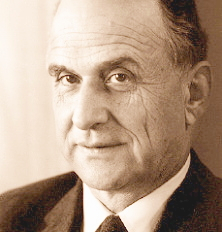
\includegraphics[width=0.74in]{img/goodman} \caption[Nelson Goodman (1906--1988) discovered the grue paradox in the $1940$s and '$50$s]{Nelson Goodman (1906--1988) discovered the grue paradox in the $1940$s and '$50$s.}\label{fig:unnamed-chunk-48}
\end{marginfigure}

\newthought{But} in the \(1940\)s, Nelson Goodman discovered a problem with the Principle of Induction. To illustrate the problem he invented a very curious concept, \emph{grue}.

There are two ways for an object to be grue. Some green things are grue, but it depends on when we first encounter them. If our first observation of a green object happens before the year \(2050\), then it's grue. So the Statue of Liberty is grue: it's a green object that was first observed before the year \(2050\) (\emph{long} before).

But if our first encounter with a green object happens in the year \(2050\) or later, then it's not grue. The same goes if we never observe it. Objects on the far side of the universe that we'll never see, or buried deep underground, are not grue.

There is a second way for an object to be grue: some blue objects are grue. Not the ones observed before \(2050\), though. Instead it's the ones that \emph{aren't} observed before \(2050\). If a blue object is observed for the first time \emph{after} \(2049\), or it's never observed at all, then it's grue. So blue sapphires that won't be mined before the year \(2050\) are grue, for example.

As usual, it helps to have a diagram:

\begin{figure}
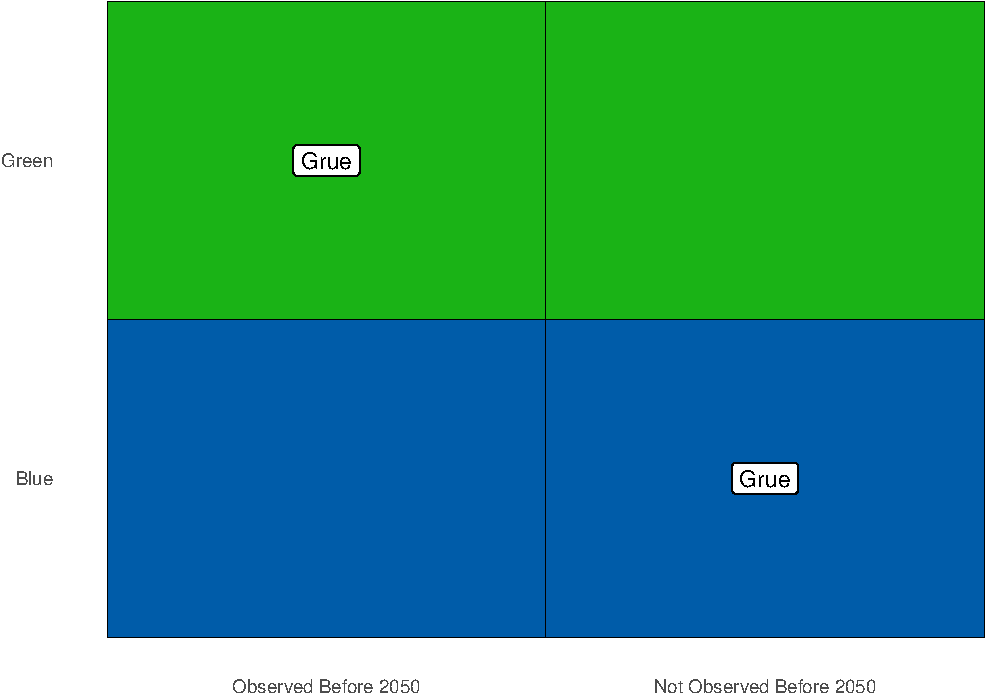
\includegraphics{_main_files/figure-latex/unnamed-chunk-49-1} \caption[The definition of grue]{The definition of grue}\label{fig:unnamed-chunk-49}
\end{figure}

Here is the formal definition of grue:

\begin{description}
\item[Grue]
An object is \emph{grue} if either (a) it is green and first observed before the year \(2050\), or (b) it's blue and not observed before \(2050\).
\end{description}

To test your understanding, see if you can explain why each of the following are examples of grue things: the \(\$20\) bill in my pocket, Kermit the Frog, the first sapphire to be mined in \(2050\), and blue planets on the far side of the universe.

Then see if you can explain why these things aren't grue: fire engines, the \href{https://en.wikipedia.org/wiki/Star_of_India_(gem)}{Star of India}, and the first \(\$20\) bill to be printed in \(2050\).

Once you've got all those down, try this question: do grue objects change colour in the year \(2050\)? It's a common mistake to think they do.

But no, grue objects don't change colour. The Statue of Liberty is green and it always will be (let's assume). So it's grue, and always will be, because it's a green thing that was first observed before the year \(2050\). Part (a) of the definition of grue guarantees that.

The only way time comes into it is in determining which green things are grue, and which blue things. If a green thing is first observed before \(2050\), then it's grue, ever and always. Likewise if a blue thing is \emph{not} first observed before \(2050\). Then it's grue---and it always has been!

\hypertarget{the-paradox}{%
\section*{The Paradox}\label{the-paradox}}
\addcontentsline{toc}{section}{The Paradox}

\newthought{Now} ask yourself, have you ever seen a grue emerald? You probably have. In fact, every emerald everyone's ever seen has been grue.

Why? Because they're all green, and they've all been observed before the year \(2050\). So they're all grue the first way---they all satisfy part (a) of the definition. (Notice it's an either/or definition, so you only have to satisfy one of the two parts to be grue.)

So all the emeralds we've ever seen have been grue. Let's apply the Principle of Induction then:

\begin{argument}
All observed emeralds have been grue.\\
Therefore \emph{all} emeralds are grue.
\end{argument}

But if all emeralds are grue, then the first emeralds to be mined in \(2050\) will be grue. And that means they'll be blue! Because they won't have been observed before \(2050\), so the only way for them to be grue is to be blue.

We've reached the absurd conclusion that there are blue emeralds out there, just waiting to be pulled out of the earth. Something has gone off the rails here, but what?

Here's another way to put the challenge. We have two ``patterns'' in our observed data. The emeralds we've seen are uniformly green, but they're also uniformly grue. We can't project both these patterns into the future, though. They'll contradict each other starting in \(2050\).

Now, obviously, common sense says the green pattern is the real one. The grue ``pattern'' is bogus, and no one but a philosopher would even bother thinking about it. But \emph{why} is it bogus? What's so special about green?

Apparently the Principle of Induction has a huge hole in it! It says to extrapolate from observed patterns. But \emph{which} patterns?

\hypertarget{grue-artificial-intelligence}{%
\section*{Grue \& Artificial Intelligence}\label{grue-artificial-intelligence}}
\addcontentsline{toc}{section}{Grue \& Artificial Intelligence}

\begin{marginfigure}
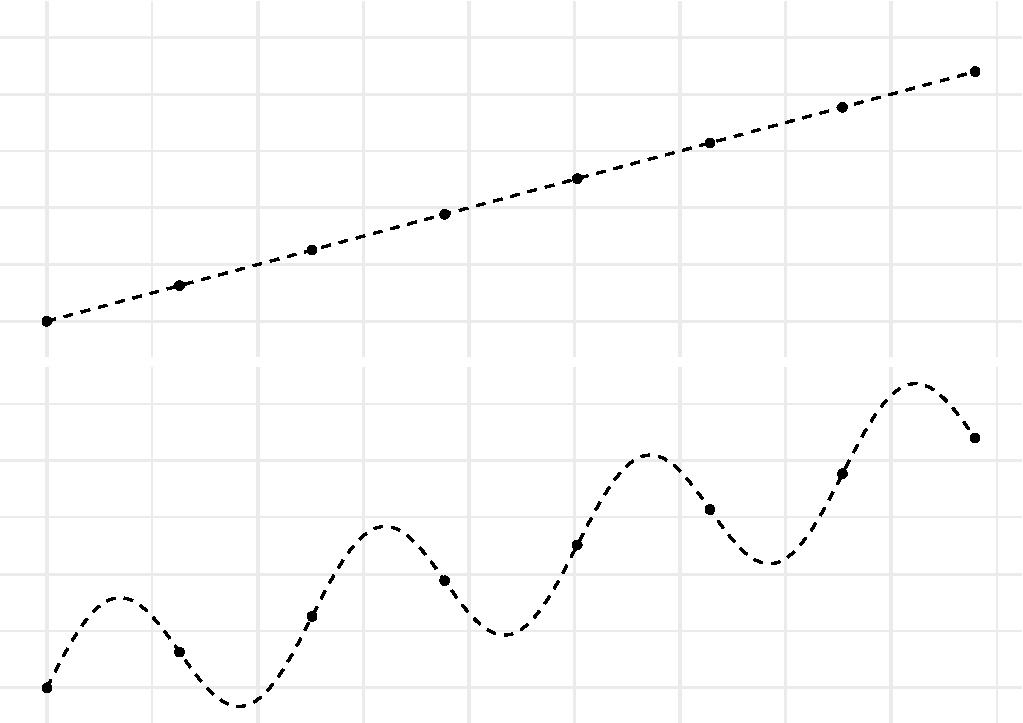
\includegraphics{_main_files/figure-latex/curvefitting-1} \caption[The same set of points interpreted two different ways]{The same set of points interpreted two different ways}\label{fig:curvefitting}
\end{marginfigure}

Patterns are cheap, as any data scientist will tell you. Given a bunch of data points in an \emph{xy}-plane, there are lots of ways to connect the dots. Even if they all lie on a straight line, you could draw an oscillating curve that passes through each point (Figure \ref{fig:curvefitting}). You can probably think of even sillier curves that will fit all the points.

Designing a computer program that will know which patterns to use and which to ignore is a big part of what machine learning experts do. And it's one reason humans are still essential to designing artificial intelligence. Thanks to our experience, and our genetic inheritance, we have \emph{lots} of information about which patterns are likely to continue, and which are bogus, like grue.

But how do we pass all that wisdom on to the machines? How do we teach them the difference between green and grue, so that they can take it from here and we can all go on permanent vacation?

\hypertarget{disjunctivitis}{%
\section*{Disjunctivitis}\label{disjunctivitis}}
\addcontentsline{toc}{section}{Disjunctivitis}

\newthought{Here's one} very natural answer. The problem with grue is that it's \emph{disjunctive}: it's defined using either/or. It suffers from what we might call ``disjunctivitis''.

But the beauty of Goodman's puzzle is the neat way it exposes the flaw in this answer. It allows us to make `green' the disjunctive concept instead! How? We start by building grue a friend, a concept to fill in the missing spaces in our original diagram. We'll call it \emph{bleen}:

\begin{figure}
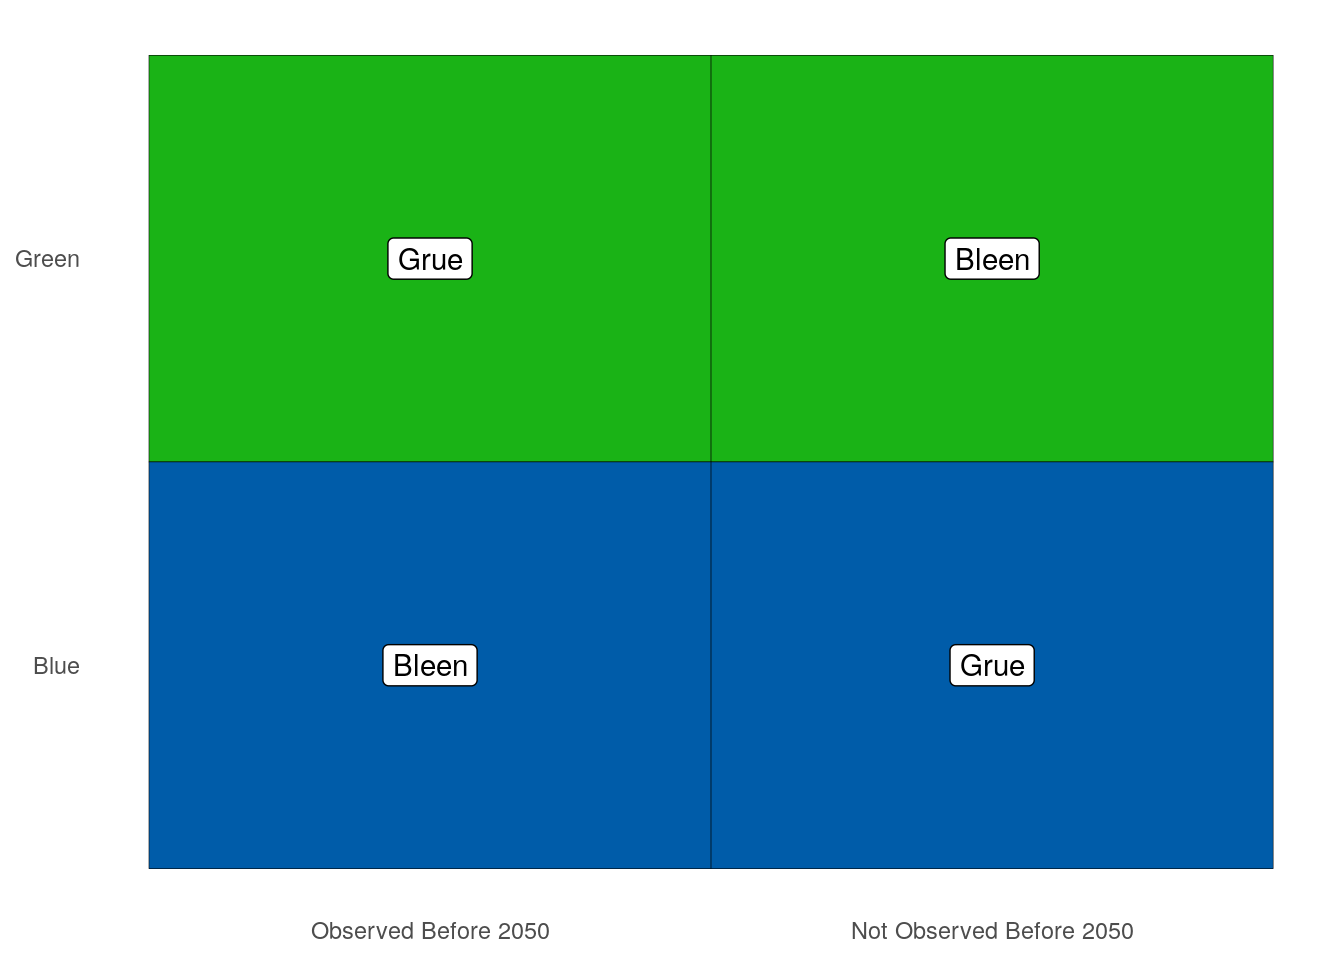
\includegraphics{_main_files/figure-latex/unnamed-chunk-51-1} \caption[Defining bleen, a counterpart to grue]{Defining bleen, a counterpart to grue}\label{fig:unnamed-chunk-51}
\end{figure}

Now we can define green in terms of grue and bleen:

\begin{description}
\item[Green]
An object is \emph{green} if either (a) it's grue and first observed before the year \(2050\), or (b) it's bleen and not observed before \(2050\).
\end{description}

Now maybe you're thinking: you \emph{could} define green that way, but that's not how it's \emph{actually} defined. In reality, we already understand the concept of green, and we have to learn the concept of grue from its disjunctive definition.

The problem is, that's just a fact about \emph{us humans}, not about the concepts grue and green. That's just the way we \emph{homo sapiens} happen to be built (or maybe socialized, or both).

Some bizarre species of alien could grow up thinking in grue/bleen terms instead. And when they landed on Earth, we'd have to explain our green/blue language to them using an either/or definition. Then \emph{they} would be looking at \emph{us} thinking: you guys have a very weird, disjunctive way of thinking!

What could we say to them to establish the superiority of our way of thinking? It's been more than \(70\) years since Goodman first posed this question. Yet no answer has emerged as the clear and decisively correct one.

\hypertarget{time-dependence}{%
\section*{Time Dependence}\label{time-dependence}}
\addcontentsline{toc}{section}{Time Dependence}

\newthought{Another} natural answer to Goodman's challenge is to say that grue is defective because it's time-dependent. It means different things depending on the time an object is first observed.

But the same reversal of fortunes that toppled the ``disjunctivitis'' diagnosis happens here. We can define green in terms of grue and bleen. And when we do, it's green that's the time-dependent concept, not grue.

So we're left in the same spot. We need some way of showing that the ``true'' order of definition is the one we're used to. By what criterion can we say that green is more fundamental, more basic, than grue?

\hypertarget{the-moral}{%
\section*{The Moral}\label{the-moral}}
\addcontentsline{toc}{section}{The Moral}

\begin{marginfigure}
\href{http://www.wi-phi.com/video/puzzle-grue}{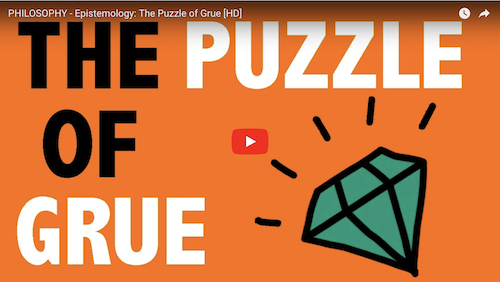
\includegraphics{img/wiphi_grue.png}}
For another explanation of the grue puzzle, check out
\href{http://www.wi-phi.com/video/puzzle-grue}{this excellent Wi-Phi
video}.
\end{marginfigure}

\newthought{Goodman's puzzle} may seem just cute at first, a mere curiosity. But it is actually quite profound.

In a way, the central question of this book is: what is the logic of science? What are the correct rules of scientific reasoning?

The laws of probability seem like a good place to start. But that path led us to a dead end at the problem of priors in \protect\hyperlink{priors}{Chapter} \ref{priors}. Perhaps then we could start with the Principle of Induction instead? But then we end up in another dead end, stopped by the grue paradox.

Just as Bertrand's paradox stops us from using the Principle of Indifference to answer the problem of priors, Goodman's paradox stops us from using the Principle of Induction.

There is even more to the similarity between these two paradoxes. Both paradoxes are problems of ``language dependence''. Depending on what language we work in, rules like the Principle of Indifference and the Principle of Induction give different recommendations. If we apply the Principle of Indifference to length, we get one prior probability; if we apply it to area, we get another. If we apply the Principle of Induction to green, we expect all emeralds to be green; if we apply it to grue, we expect some to be blue.

To this day, we do not have an answer to the question: which language is the right one to use, and why?

\hypertarget{the-problem-of-induction}{%
\chapter{The Problem of Induction}\label{the-problem-of-induction}}

\newthought{Many} inductive arguments work by projecting an observed pattern onto as-yet unobserved instances. All the ravens we've observed have been black, so all ravens are. All the emeralds we've seen have been green, so all emeralds are.

The assumption that the unobserved will resemble the observed seems to be central to induction. Philosophers call this assumption the \emph{Principle of Induction}.\footnote{See \protect\hyperlink{indargs}{Section} \ref{indargs} and \protect\hyperlink{grue}{Appendix} \ref{grue} for previous discussions of the Principle of Induction.} But what justfies this assumption? Do we have any reason to think the parts of reality we've observed so far are a good representative of the parts we haven't seen yet?

Actually there are strong reasons to doubt whether this assumption can be justified. It may be impossible to give any good argument for expecting the unobserved to resemble the observed.

\hypertarget{the-dilemma}{%
\section*{The Dilemma}\label{the-dilemma}}
\addcontentsline{toc}{section}{The Dilemma}

\newthought{We} observed previously that there are two kinds of argument, inductive and deductive. Some arguments establish their conclusions necessarily, others only support them with high probability. If there is an argument for the Principle of Induction, it must be one of these two kinds. Let's consider each in turn.

Could we give an inductive argument for the Principle of Induction? At first it seems we could. Scientists have been using inductive reasoning for millenia, often with great success. Indeed, it seems humans, and other creatures too, have relied on it for much longer, and could not have survived without it. So the Principle of Induction has a very strong track record. Isn't that a good argument for believing it's correct?

\begin{marginfigure}
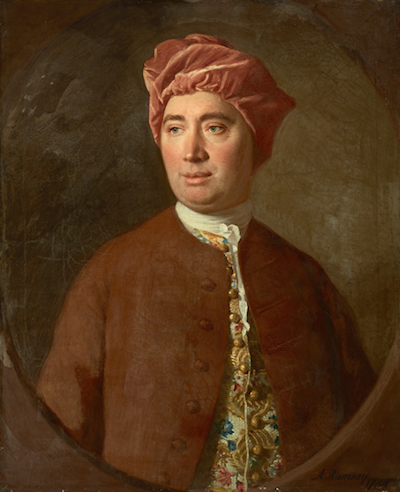
\includegraphics[width=1.33in]{img/hume} \caption[David Hume (1711--1776) raised the problem of induction in $1739$]{David Hume (1711--1776) raised the problem of induction in $1739$. Our presentation of it here is somewhat modernized from his original argument.}\label{fig:unnamed-chunk-53}
\end{marginfigure}

No, because the argument is circular. It uses the Principle of Induction to justify believing in the Principle of Induction. Consider that the argument we are attempting looks like this:

\begin{argument}
The principle has worked well when we've used it in the past.\\
Therefore it will work well in future instances.
\end{argument}

This is an inductive argument, an argument from observed instances to ones as yet unobserved. So, under the hood, it appeals to the Principle of Induction. But that's exactly the conclusion we're trying to establish. And one can't use a principle to justify itself.

What about our second option: could a deductive argument establish the Principle of Induction? Well, by definition, a deductive argument establishes its conclusion with necessity. Is it necessary that the unobserved will be like the observed? It doesn't look like it. It seems perfectly possible that tomorrow the world will go haywire, randomly switching from pattern to pattern, or even to no pattern at all.

Maybe tomorrow the sun will fail to rise. Maybe gravity will push apart instead of pull together, and all the other laws of physics will reverse too. And just as soon as we get used to those patterns and start expecting them to continue, another pattern will arise. And then another. And then, just as we give up and come to have no expectation at all about what will come next, everything will return to normal. Until we get comfortable and everything changes again.

Thankfully, our universe hasn't been so mischievous. We get surprised now and again, but for the most part inductive reasoning is pretty reliable, when we do it carefully. But we're lucky in this respect, is the point.

Nature \emph{could} have been mischievous, totally unpredictable. It is not a necessary truth that the unobserved must resemble the observed. And so it seems there cannot be a deductive argument for the Principle of Induction. Because such an argument would establish the principle as a necessary truth.

\hypertarget{the-problem-of-induction-vs.the-grue-paradox}{%
\section*{The Problem of Induction vs.~the Grue Paradox}\label{the-problem-of-induction-vs.the-grue-paradox}}
\addcontentsline{toc}{section}{The Problem of Induction vs.~the Grue Paradox}

\newthought{If} you read \protect\hyperlink{grue}{Appendix} \ref{grue}, you know of another famous problem with the Principle of Induction: the grue paradox. (If you haven't read that chapter, you might want to skip this section.)

The two problems are quite different, but it's easy to get them confused. The problem we're discussing here is about justifying the Principle of Induction. Is there any reason to believe it's true? Whereas the grue paradox points out that we don't even really know what the principle says, in a way. It says that what we've observed is a good indicator of what we haven't yet obsered. But in what respects? Will unobserved emeralds be green, or will they be grue?

So the challenge posed by grue is to spell out, precisely, what the Principle of Induction says. But even if we can meet that challenge, this challenge will remain. Why should we believe the principle, once it's been spelled out? Neither a deductive argument nor an inductive argument seems possible.

\hypertarget{probability-theory-to-the-rescue}{%
\section*{Probability Theory to the Rescue?}\label{probability-theory-to-the-rescue}}
\addcontentsline{toc}{section}{Probability Theory to the Rescue?}

\newthought{The} Problem of Induction is centuries old. Isn't it out of date? Hasn't the modern, mathematical theory of probability solved the problem for us?

Not at all, unfortunately. One thing we learn in this book is that the laws of probability are very weak in a way. They don't tell us much, without us first telling them what the prior probabilities are. And as we've seen over and again throughout Part III, \protect\hyperlink{priors}{the problem of priors} is very much unsolved.

For example, suppose we're going to flip a mystery coin five times. We don't know whether the coin is fair or biased, but we hope to have some idea after a few flips.

Now suppose we get through the first four flips and they've all been tails. The Principle of Induction says we should expect the next flip to be tails too. At least, that outcome should now be more probable.

Do the laws of probability agree? Well, we need to calculate the quantity:
\[ \p(T_5 \given T_1 \wedge T_2 \wedge T_3 \wedge T_4).\]
The definition of conditional probability tell us:
\[
  \begin{aligned}
    \p(T_5 \given T_1 \wedge T_2 \wedge T_3 \wedge T_4) 
      &= \frac{\p(T_1 \wedge T_2 \wedge T_3 \wedge T_4 \wedge T_5)}
              {\p(T_1 \wedge T_2 \wedge T_3 \wedge T_4)}.
  \end{aligned}
\]
But the laws of probability don't tell us what numbers go in the numerator and the denominator.

The numbers have to be between \(0\) and \(1\). And we have to be sure mutually exclusive propositions have probabilities that add up, according to the Additivity rule. But that still leaves things wide open.

For example, we could finish the calculation this way:
\[
  \begin{aligned}
    \p(T_5 \given T_1 \wedge T_2 \wedge T_3 \wedge T_4) 
      &= \frac{\p(T_1 \wedge T_2 \wedge T_3 \wedge T_4 \wedge T_5)}
              {\p(T_1 \wedge T_2 \wedge T_3 \wedge T_4)}\\
      &= \frac{1/32}{1/16}\\
      &= 1/2.
  \end{aligned}
\]
Or we could finish it this way:
\[
  \begin{aligned}
    \p(T_5 \given T_1 \wedge T_2 \wedge T_3 \wedge T_4) 
      &= \frac{\p(T_1 \wedge T_2 \wedge T_3 \wedge T_4 \wedge T_5)}
              {\p(T_1 \wedge T_2 \wedge T_3 \wedge T_4)}\\
      &= \frac{5/20}{6/20}\\
      &= 5/6.
  \end{aligned}
\]
We could even do this:
\[
  \begin{aligned}
    \p(T_5 \given T_1 \wedge T_2 \wedge T_3 \wedge T_4) 
      &= \frac{\p(T_1 \wedge T_2 \wedge T_3 \wedge T_4 \wedge T_5)}
              {\p(T_1 \wedge T_2 \wedge T_3 \wedge T_4)}\\
      &= \frac{0}{1}\\
      &= 0.
  \end{aligned}
\]

All these options result from different choices of prior probabilities. And the laws of probability don't tell us what prior probabilities we must choose, as we learned in Part III.

So the laws of probability don't by themselves tell us what to expect. It could be undecided, with heads and tails equally probable on the final toss (\(1/2\)). Or the pattern of tails could continue into the future with high probability (\(5/6\)). There could even be no chance of the pattern continuing (\(0\)).

The laws of probability only tell us what to expect once we've specified the necessary prior probabilities. The problem of induction challenges us to justify one choice of prior probabilities over the alternatives.

In the \(280\) years since this challenge was first raised by David Hume, no answer has gained general acceptance.



\end{document}
